\documentclass[a4paper,12pt]{article}

\usepackage[unicode]{hyperref}
\usepackage{cmap}
\usepackage[T2A]{fontenc}
\usepackage[utf8]{inputenc}


\usepackage[verbose,dvips,a4paper,tmargin=20mm,bmargin=20mm,lmargin=20mm,rmargin=20mm,headsep=4pt,includeheadfoot]{geometry}

\usepackage[nodisplayskipstretch]{setspace}
\usepackage{amsmath}
%\usepackage{mathenv}
\usepackage{mathtools}
\usepackage{indentfirst}
\usepackage{titling}

\usepackage{txfonts} % use before local fonts - only for math
%\usepackage{dejavu}
\usepackage{atu_csb}
\usepackage{atu_ofs}
\usepackage{atu_nim}

\usepackage{graphicx}
\usepackage{placeins} % FloatBarrier
\usepackage{siunitx}

\usepackage{tikz}
\usetikzlibrary{arrows}
\usetikzlibrary{patterns}

\usepackage{blox}
\usepackage[europeanresistors,americaninductors,siunitx,fulldiodes]{circuitikz}

\usetikzlibrary{calc}
\usetikzlibrary{arrows}
\usetikzlibrary{patterns}
%\usepgflibrary{shapes.geometric}
\usetikzlibrary{external}


\definecolor{haircolor}{rgb}{0.7,0.7,1.0}
\newcommand{\TikzAddPadding}{\path (current bounding box.north east) ++(+0.1,+0.1); \path (current bounding box.south west) ++(-0.1,-0.1);}

\tikzset{
  >=stealth,
  %semiRed/.style={fill=red,opacity=0.3,draw=black,thin},
  hair/.style={draw,color=haircolor,line width=0.1pt},
  medline/.style={draw=black,line width=0.6pt},
  medlinep/.style={draw=black,line width=0.6pt,->},
  semiboldline/.style={draw=black,line width=1.2pt},
  semiboldlinep/.style={draw=black,line width=1.2pt,->},
  infoline/.style={draw=gray,line width=1.4pt},
  boldline/.style={draw=black,line width=2.0pt},
  boldlinep/.style={draw=black,line width=2.0pt,->},
  wire/.style={draw=black,line width=1.0pt},
  elelem/.style={draw=black,line width=1.5pt},
  subelem/.style={draw=black,dashed,line width=0.6pt}
}


\usepackage[europeanresistors,americaninductors,siunitx,fulldiodes]{circuitikz}

\usepackage[english,ukraineb,russian]{babel}
%\usepackage[margin=10pt,font=small,labelfont=bf,labelsep=endash]{caption} % format=hang|plain...

\usepackage{currfile}

\setcounter{topnumber}{3}
\renewcommand\topfraction{.7}
\setcounter{bottomnumber}{2}
\renewcommand\bottomfraction{.6}
\setcounter{totalnumber}{7}
\renewcommand\textfraction{.1}
\renewcommand\floatpagefraction{.5}
\setcounter{dbltopnumber}{2}
\renewcommand\dbltopfraction{.7}
\renewcommand\dblfloatpagefraction{.6}

\clubpenalty9500
\widowpenalty9500%


\newlength{\TW}
\setlength{\TW}{0.01\textwidth}

\DeclareMathOperator*{\sign}{sign}

\title{Идентификация хаотических систем}
\author{А.И.~Гуда}

\hypersetup{
  pdftitle={\thetitle},
  pdfauthor={\theauthor},
  colorlinks=true,
  linkcolor=blue,
  citecolor=brown
}

% \linespread{1.3} setspace must be better
% \onehalfspacing
\setstretch{1.2}

\newcommand{\LinkRef}[1]{ \textit{\color{red}#1} }
\newcommand{\Cmt}[1]{ {\small\color{red}#1} }


\begin{document}

% \maketitle
%{ \tiny \verb! ~/proj/id_data/text/tasks.tex! }
{ \tiny \currfilepath }

\tableofcontents


\section{Определение идентификации}

\subsection{История}

\Cmt{Предельные случаи: Заде, Райбман.}

L.A.~Zadeh (1956), ``On the Identification Problem,''
IRE Transactions on Circuit Theory, 3, pp.  277--281.

More: Eykhoff, Rastrigin.

\subsection{Новые определения}

\Cmt{Привязка к текущей задаче, физика.}

\Cmt{Разные определения для разных задач или свести к одному определению?}

\subsection{Критерии идентификации}

\subsubsection{Отличие задачи идентификации от поиска экстремума}

На первый взгляд, при заданном критерии идентификации, задача идентификации
сводится к классической задаче описка экстремума: надо найти такие значения
параметров, при которых критерий принимает максимальное значение.
На самом деле, существуют определённые аспекты, которые делают такое
сведение практически невозможным.

Прежде всего, в задаче поиска
экстремума предполагается, что наблюдаемая система статична:
значение критерия не зависит от времени, и проведя измерение
в точке один раз, можно к нему не возвращаться.
Напротив, идентификация динамической системы предполагает,
что значение критерия, даже после какого-либо усреднения на конечном
интервале времени, есть величина динамическая, причём динамика определяется
не только параметрами системы, но и свойствами самой системы измерения,
а также процессом взаимодействия системы измерения с моделями. При этом
возможны весьма нетривиальные результаты, такие как параметрический
резонанс, распространение параметрических волн на множестве моделей и т.д.

Также существенную роль могут играть как шумы измерения, так и побочные
эффекты от процесса фильтрации шумов. Большая часть фильтров приводит к запаздыванию
в процессе измерения, и игнорирование этих явлений может привести
к нарушению устойчивости поиска.

В задаче поиска экстремума предполагается, что не только
значение функции известно точно в каждой точке, но также известны все производные.
В реальные задачах идентификации производные непосредственно
не доступны для измерения, а их оценка требует применения специальных
методов. При этом процесс оценивания производных, как правило,
более чувствителен к шумам измерения, чес собственно измерение.

Далее, в в задачах поиска экстремума не учитывается возможность
смещения экстремума со временем. Напротив, в задачах идентификации
или же изначально предполагается вариабельность параметров, или же
имеются ограничение на время измерения.


Все эти явления делают задачу идентификации более сложной, чем
классическая задача поиска экстремума, чем и обусловлено
существование широкого спектра методов идентификации. Тем не менее,
некоторые алгоритмы, применимые при поиска экстремума, могут быть
полезны при синтезе системы идентификации.






\subsubsection{Измеримые интегральные характеристики сигнала}

Откуда брать.


\subsection{Тестовые системы (хаотические)}

\subsubsection{Система Лоренца} % _LOR_

\LinkRef{
  lor: ASAU-22, 23, 24, 25, 26. APIR-2012. CSIT-2015. ISDMCI-2014, ISDMCI-2015.
  ITMM-2012, ITMM-2014, ITMM-2015, DSMP-2016
}

В качестве первой идентифицируемой хаотической системы рассмотрим
систему Лоренса, динамика которой описывается системой уравнений~[??]:

\begin{equation}
\begin{cases}
  \dot{x} = \sigma (y-x ) , \\
  \dot{y} = x (r-z) - y , \\
  \dot{z} = x y - b z .
\end{cases}
\label{atu:eq:lor}
\end{equation}

Наиболее ценным с точки зрения идентификации является параметр
$r$, определяющий как энергетическое состояние системы,
так и вид динамики системы.
Для определённости зададим остальные параметры следующим образом:
$b = 2.6666667$, $\sigma = 10$.

Критерий
$\overline{x^2}$


% Идентифицируемый параметр:
% $r \in [ 5; 100 ] $.
%
% Остальные параметры:
% $b = 2.66667$, $\sigma = 10$.


\begin{figure}[htb!]
\centerline{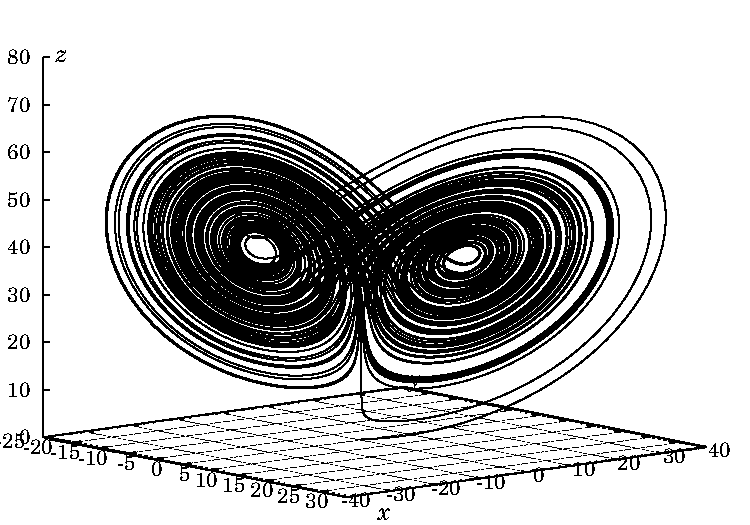
\includegraphics[width=0.5\textwidth]{p/cha/lor_phase3.pdf} }
\caption{Аттрактор системы Лоренца (\ref{atu:eq:lor})}
\label{atu:f:lor_phase}
\end{figure}


\FloatBarrier
\subsubsection{Система Дуффинга} % _DUFF_

\LinkRef{
 duff: ASAU-12, 15. APIR-2009. DSMP-2016
}

\begin{equation}
 \ddot{x} + c_0 \dot{x} + \Omega_0^2 x + \beta x^3 = u(t) ,
\label{atu:eq:duff}
\end{equation}

\begin{equation}
 m \ddot{x} + \nu \dot{x} + k_1 x + k_3 x^3 = F(t) ,
\label{atu:eq:duff_phys}
\end{equation}

Здесь \(m\) -- масса объекта,
\(x(t)\) -- координата (выходной сигнал),
\(u(t) = U_{in} \sin( \omega_{in} t ) \) -- внешняя возмущающая сила,
\( k_1 \) -- коэффициент линейной компоненты возвращающей силы,
\( k_3 \) -- коэффициент при нелинейной части,
\( \Omega_0 \) -- собственная частота при отсутствии нелинейности,
\( \nu \) и \( c_0\) -- размерный и безразмерный коэффициенты демпфирования,
\( \beta \) -- безразмерный коэффициент нелинейной части.

Идентифицируемый параметр:
$ \beta \approx 2 $.

Остальные параметры:
\(U_{in}=1\), \(\omega_{in}=1\),
\(c_0 = 0.05\), \( \Omega_0 = 1 \).

\begin{figure}[htb!]
\centerline{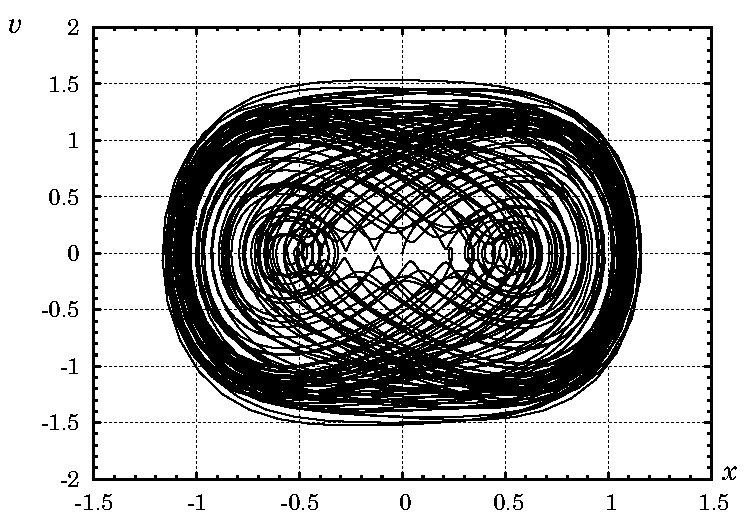
\includegraphics[width=0.5\textwidth]{p/cha/duff_phase.pdf} }
\caption{Фазовый портрет системы Дуффинга (\ref{atu:eq:duff})}
\label{atu:f:duff_phase}
\end{figure}

Критерий
$\overline{x^2}$




\FloatBarrier
\subsubsection{Система Чуа} % _CHUA_

\LinkRef{
 chua: ASAU-18, MKMM-2014, APIR-2011
}

Одной из известных хаотических систем, легко реализуемых как модельно,
так и схемотехнически (рис.~\ref{atu:f:chuascheme}),
является нелинейная система Чуа~[??]:

\begin{figure}[htb!]
\begin{center}
% vi:syntax=tex

\begin{circuitikz}[line width=0.7]
  \ctikzset{bipoles/thickness=2}
  \def\Top{3.0}
  \draw (0.0,0.0) to[L,l=$L$,i=$I_L$] (0,\Top)
   to[R=R] (6.0,\Top)
   to[ageneric,l=$R_c$] (6.0,0.0) -- (0.0,0.0);
  \draw(1.5,0.0) to[C,l=$C_2$,v=$V_2$] (1.5,\Top );
  \draw(4.5,0.0) to[C,l=$C_1$,v=$V_1$] (4.5,\Top );
\end{circuitikz}

% \begin{tikzpicture}[circuit ee IEC,very thick,circuit symbol unit=3.5mm]
%   \node (L1) at (0,1.5) [point up,elelem,inductor={info = $L$}] {};
%   \node      at (0.2,2.4) {$I_L$};
%   \node (C2) at (1.5,1.5) [point up,elelem,capacitor={info = $C_2$}] {};
%   \node      at (1.8,1.8) {$V_2$};
%   \node (pc2d) at (1.5,0) [contact] {};
%   \node (pc2u) at (1.5,3) [contact] {};
%   \node (C1) at (5.0,1.5) [point up,elelem,capacitor={info = $C_1$}] {};
%   \node      at (5.3,1.8) {$V_1$};
%   \node (pc1d) at (5,0) [contact] {};
%   \node (pc1u) at (5,3) [contact] {};
%   \node (R) at (3,3) [elelem,resistor={info = $R$}] {};
%   \node (Rc) at (7,1.5) [elelem,point up,resistor={info = $R_c$}] {};
%   \draw (Rc) ++(-0.15,-0.7) rectangle+(0.3,0.2);
%   \draw (L1) |- (pc2d) -- (pc1d) -| (Rc) [wire];
%   \draw (L1) |- (pc2u) -- (R) -- (pc1u) -| (Rc) [wire];
%   \draw (pc2u) -- (C2) [wire]; \draw (pc2d) -- (C2) [wire];
%   \draw (pc1u) -- (C1) [wire]; \draw (pc1d) -- (C1) [wire];
%   \node (Gr) at (5,-0.3) [elelem,point down,ground] {};
%   \draw (pc1d) -- (Gr) [wire];
% \end{tikzpicture}

\end{center}
\caption{Условная электрическая цепь, реализующая хаотическую систему Чуа}
\label{atu:f:chuascheme}
\end{figure}


\begin{equation}
\begin{cases}
  C_1 \dot{V_1}  = \frac{1}{R} ( V_2 - V_1 ) - g(V_1), \\
  C_2 \dot{V_2}  = \frac{1}{R} ( V_1 - V_2 ) + I_L, \\
  \dot{I_L}      = - \frac{1}{L} V_2 .
\end{cases}
\label{atu:eq:chua}
\end{equation}

Единственным нелинейным элементом в данной системе является ``диод Чуа''
(обозначен на схеме как $R_c$) с
характеристикой $g(V)$~(рис.~\ref{atu:f:diodchua}),
обладающий различным отрицательным наклоном
($m_0$ и $m_1$) на разных участках,
тем самым являющийся управляемым источником энергии.


\begin{equation}
g(V) =
\begin{cases}
  m_1 V = ( m_0 + m_2 ) V & |V| <   U_0, \\
  m_0 V                   & |V| \ge U_0.
\end{cases}
\label{atu:eq:diodchua}
\end{equation}

\begin{figure}[htb!]
\begin{center}
% vi:syntax=tex
\begin{tikzpicture}
  \coordinate (XMIN) at (-4.5,0.0);
  \coordinate (XMAX) at ( 4.5,0.0);
  \coordinate (YMIN) at (0,-2.5);
  \coordinate (YMAX) at (0, 2.5);
  \draw (XMIN) -- (XMAX) [medline,->] node[below] {$U$};
  \draw (YMIN) -- (YMAX) [medline,->] node[left]  {$I$};
  \draw (-4,2) -- (-1,1) -- (1,-1) -- (4,-2) [boldline];
  \draw (1,-1) -- (1,0) [dashed,medline];
  \draw (1,-1) -- (4,-1) [dashed,medline];
  \draw (1.41,0) arc [medline,->,start angle=0,end angle=-45,radius=1.41];
  \draw (1,-1) ++(2,0) arc [medline,->,start angle=0,end angle=-18,radius=2.0];
  \filldraw (1,0) circle[radius=0.05,fill=black] node[above] {$U_0$};
  \node[right] at (1.2,-0.6) {$\alpha_1: \tan(\alpha_1)=m_1$};
  \node[right] at (3.0,-1.3) {$\alpha_0$};
\end{tikzpicture}

\end{center}
\caption{Характеристика \(I=g(V)\) диода Чуа}
\label{atu:f:diodchua}
\end{figure}


При этом, параметр \(m_0\) определяет поступление энергии в систему
при больших амплитудах \(V_1\), и, в целом, характеризует
энергетические возможности источника.
Аналогично, параметр \(m_1\) определяет поступление энергии
при малых колебаниях, в частности, определяет, будет ли
система переходить в колебательное состояние при малых начальных
возмущениях, и какой будет режим этих колебаний.
С другой стороны, параметр \(m_1\) является суммой
``глобального параметра'' \(m_0\) и ``довеска'',
определяющего дополнительный вклад при малых амплитудах,
то имеет смысл перейти от параметра \(m_1\) к параметру
\( m_2 = m_1 - m_0 \), который тем самым, в целом
и определяет нелинейность
системы. При \( m_2 = 0 \) система становится линейной
и не представляет особого интереса. Поэтому
в данной работе в качестве
идентифицируемого параметра рассматривается параметр \(m_2\).

В зависимости от величины этого параметра,
система может переходить в режимы затухания,
периодического и сложно-периодического движения, а также в режим
хаотических колебаний. При этом сложно-периодическое и хаотическое
движения чередуются с изменением величины \(m_2\).


Классически параметры задаются следующим образом~[chua]:
$C_1 = 1/9$, $C_2 = 1$, $L= 1/7$, $R = 1/0.7$, $m_0=-0.5$, $ m_2 \in [ -0.15; -0.7 ] $.

Введём обозначения:
\[
  a_{11} = \frac{1}{R C_1}; \;
  a_{13} = \frac{1}{C_1}; \;
  a_{21} = \frac{1}{R C_2}; \;
  a_{23} = \frac{1}{C_2}; \;
  a_{31} = -\frac{1}{L}; \;
  a_g = - \frac{m_0}{C_1}; \;
  \mu = - \frac{m_2}{C_1}.
\]

\noindent
Получаем:

\begin{equation}
\begin{cases}
  \dot{V}_1  = -a_{11} V_1 + a_{11}  V_2  + g_1(V_1) , \\
  \dot{V}_2  = +a_{21} V_1 - a_{21}  V_2  + a_{23} I_L    , \\
  \dot{I}_L  =  a_{31} V_2.
\end{cases}
\label{atu:eq:chua2}
\end{equation}


\begin{equation}
g_1(V) =
\begin{cases}
  ( a_g + \mu ) V , & |V| <   U_0, \\
  a_g V           , & |V| \ge U_0.
\end{cases}
\label{atu:eq:diodchua2}
\end{equation}

При этом классические значения параметров будут представлены следующим образом:
$ a_{11} = 6.5 $, $a_{21} = 0.7$, $ a_{23} = -7 $, $ a_g = 4.5 $,
$ \mu \in [ 1.29 ; 5.6 ] $.
Соответственно, в этих обозначениях
идентифицируемым параметров является $\mu$.



\begin{figure}[htb!]
\centerline{
  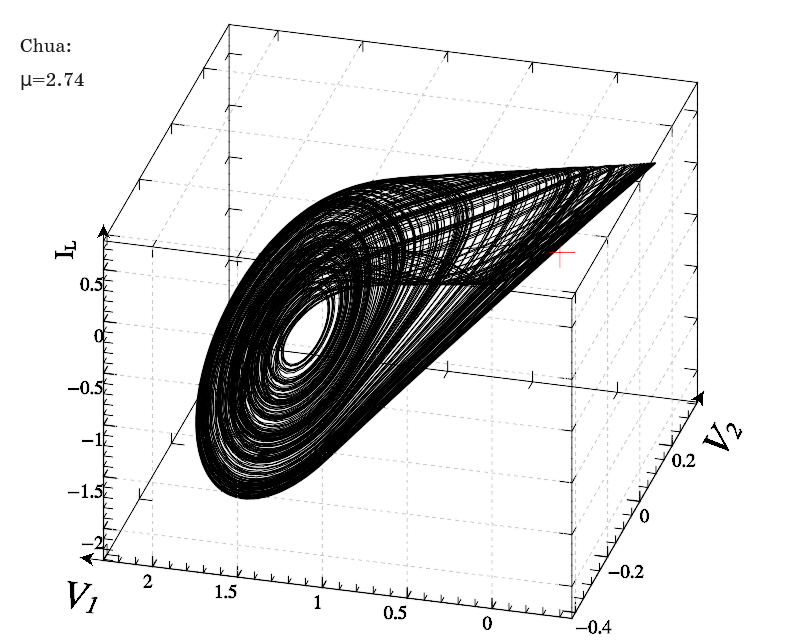
\includegraphics[width=0.49\textwidth]{p/cha/chua/chua_1-p_xyz_mu=2x74.png}
  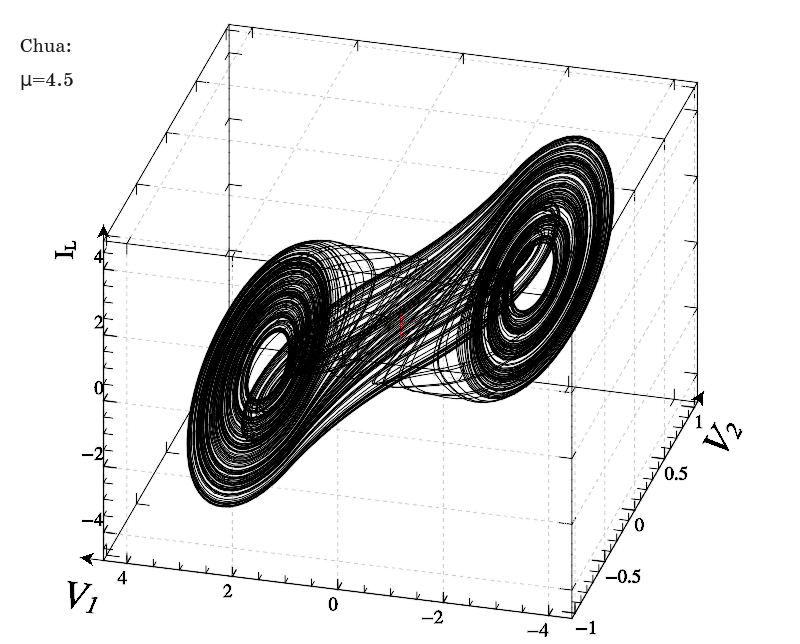
\includegraphics[width=0.49\textwidth]{p/cha/chua/chua_1-p_xyz_mu=4x50.png}
}
\caption{Аттрактор системы Чуа (\ref{atu:eq:chua2}) при различных значениях $\mu$}
\label{atu:f:chua_phase}
\end{figure}


Для определения критерия рассмотрим зависимости
$q_{*}(\mu) $, полученные путём моделирования
для системы Чуа (рис.~\ref{atu:f:chua_q}):

\begin{figure}[htb!]
\centerline{
  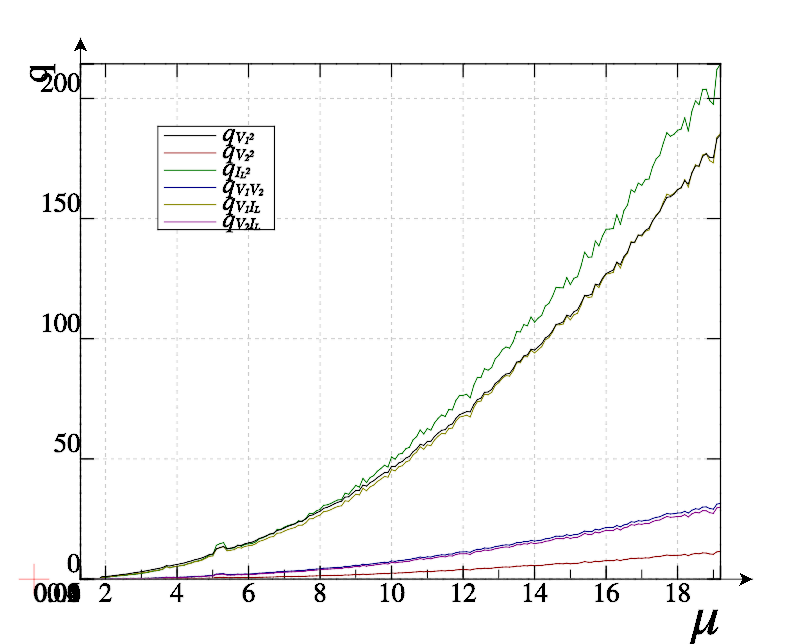
\includegraphics[width=0.49\textwidth]{p/cha/chua/chua_q-p_mu2.png}
  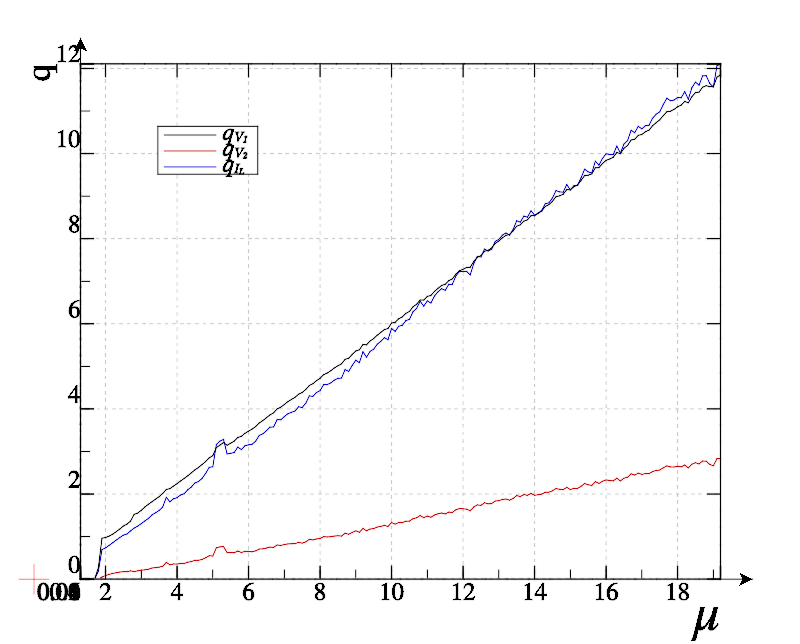
\includegraphics[width=0.49\textwidth]{p/cha/chua/chua_q-p_mu1.png}
}
  \caption{Зависимости $q_{*}(\mu) $ для системы Чуа (\ref{atu:eq:chua2})}
\label{atu:f:chua_q}
\end{figure}

Из графиков очевидно, что величина $ q_{V_1}(\mu) $
является наилучшим кандидатом в критерии, ввиду близкой к линейной зависимости
в рабочем диапазоне.

% TODO: общие слова перенести к первой системе.
Следующим важным параметром, необходимым для системы идентификации, является
характерное время время оценивания $\tau$, или же обратная ему величина $a_q$,
входящая в (). %TODO

Для предварительного оценивания величины $a_q$ рассмотрим спектры системы при различных
$\mu$ (рис.~\ref{atu:f:chua_spectrum}). Как следует из графиков, спектр системы достаточно
ограничен сверху, однако, в хаотическом режиме является сплошным практически до нуля.
Это не даёт возможности непосредственно определить $a_q$ исходя из спектра,
однако, первые существенные пики наблюдаются при $ \omega \approx 0.3 $, следовательно,
первоначальное значение $a_q$ можно оценить как $ a_q \approx 0.3 / \pi \approx 0.1 $.


\begin{figure}[htb!]
\centerline{
  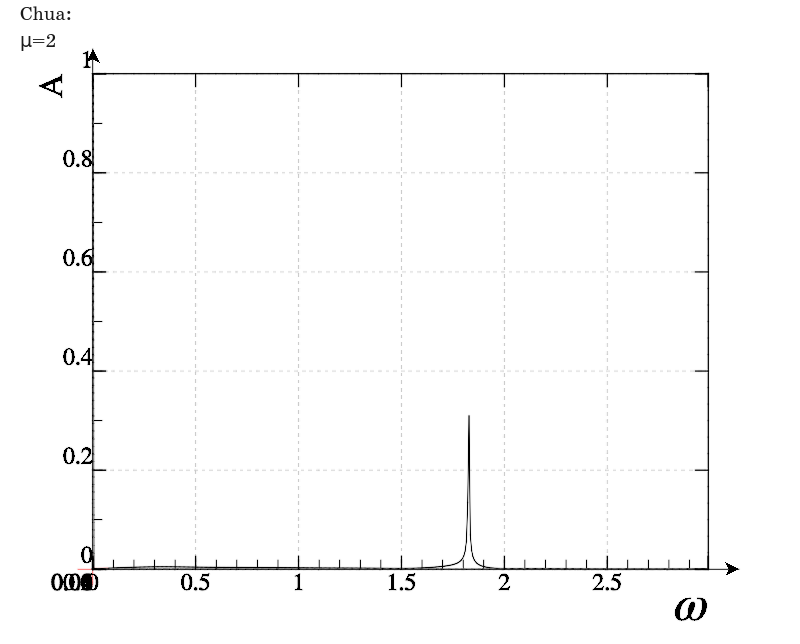
\includegraphics[width=0.32\textwidth]{p/cha/chua/chua_f-p_f_mu=2x00.png}
  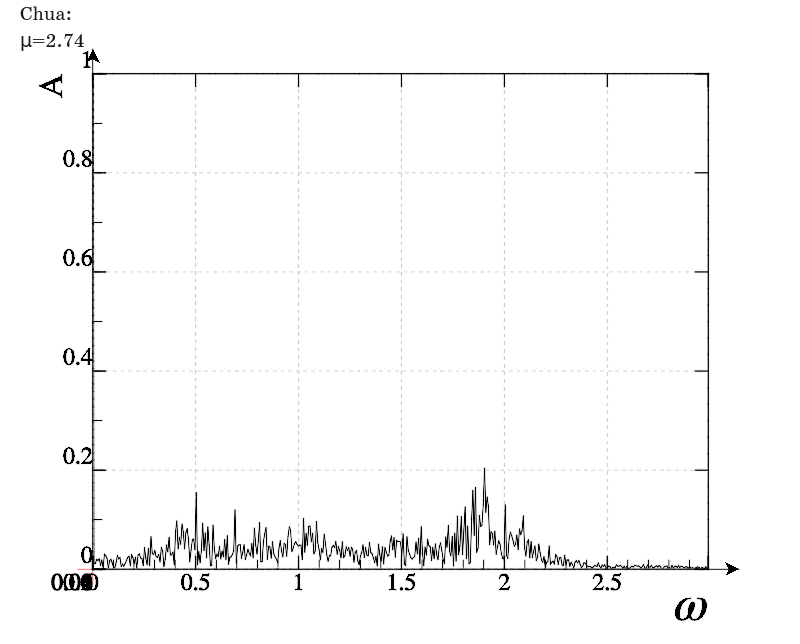
\includegraphics[width=0.32\textwidth]{p/cha/chua/chua_f-p_f_mu=2x74.png}
  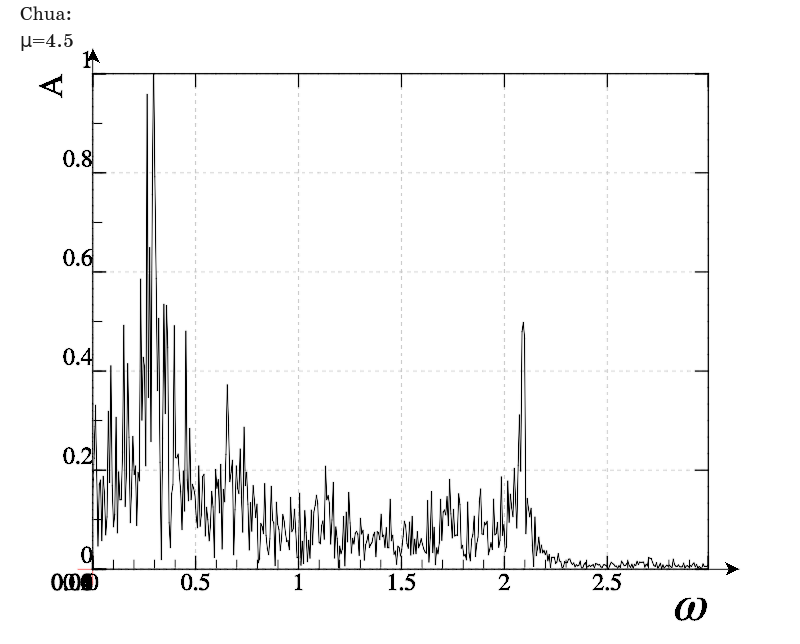
\includegraphics[width=0.32\textwidth]{p/cha/chua/chua_f-p_f_mu=4x50.png}
}
\caption{Спектры системы Чуа (\ref{atu:eq:chua2}) при различных значениях $\mu$}
\label{atu:f:chua_spectrum}
\end{figure}

Следующий способ оценить $a_q$ -- исследовать полученную в результате моделирования
зависимость среднеквадратичного отклонения $e_q$ оценки величины $q$, нормированной
на саму величину $q$ в стационарном случае. Полученная зависимость представлена
на рис.~\ref{atu:f:chua_tau}.

\begin{figure}[htb!]
\centerline{
  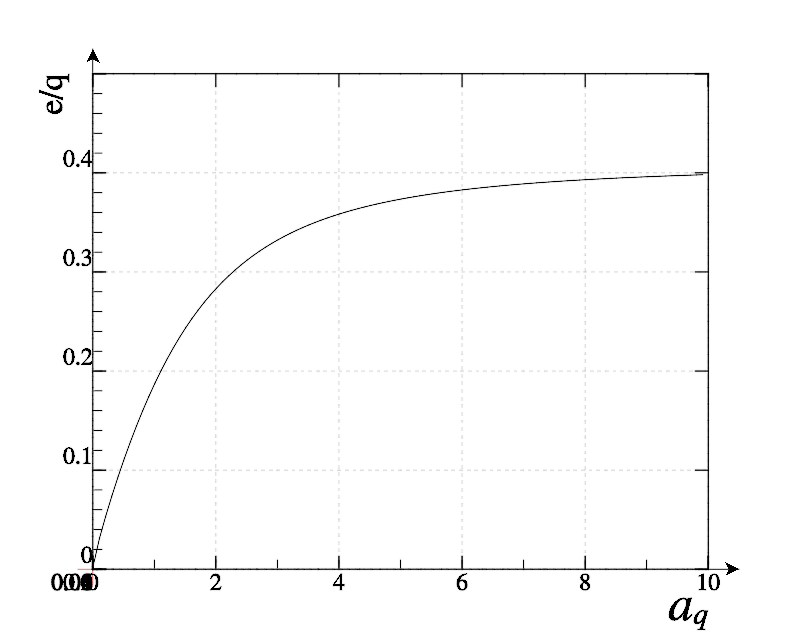
\includegraphics[width=0.4\textwidth]{p/cha/chua/chua_tau-p_e_a.png}
}
\caption{Типичная зависимость $e_q/q(a_q)$ для системы (\ref{atu:eq:chua2})}
\label{atu:f:chua_tau}
\end{figure}

Из этого графика можно сделать вывод, что первоначальная оценка $a_q$
была сделана корректно.

В качестве системы идентификации использовалась система с 5 поисковыми агентами и
двумя неподвижными моделями. Для исследования динамических свойств системы идентификации
параметр $\mu_o$ для объекта задавался двумя способами:

\begin{equation}
 \mu_o(t) = p_0 + U_p \sign \sin( \omega_p t ),
  \label{atu:eq:chua_mu_sign}
\end{equation}

\begin{equation}
 \mu_o(t) = p_0 + U_p \sin( \omega_p t ).
  \label{atu:eq:chua_mu_sin}
\end{equation}

Динамика процессов идентификации для системы Чуа представлена на рис.~\ref{atu:f:chua_id}.


\begin{figure}[htb!]
\centerline{
  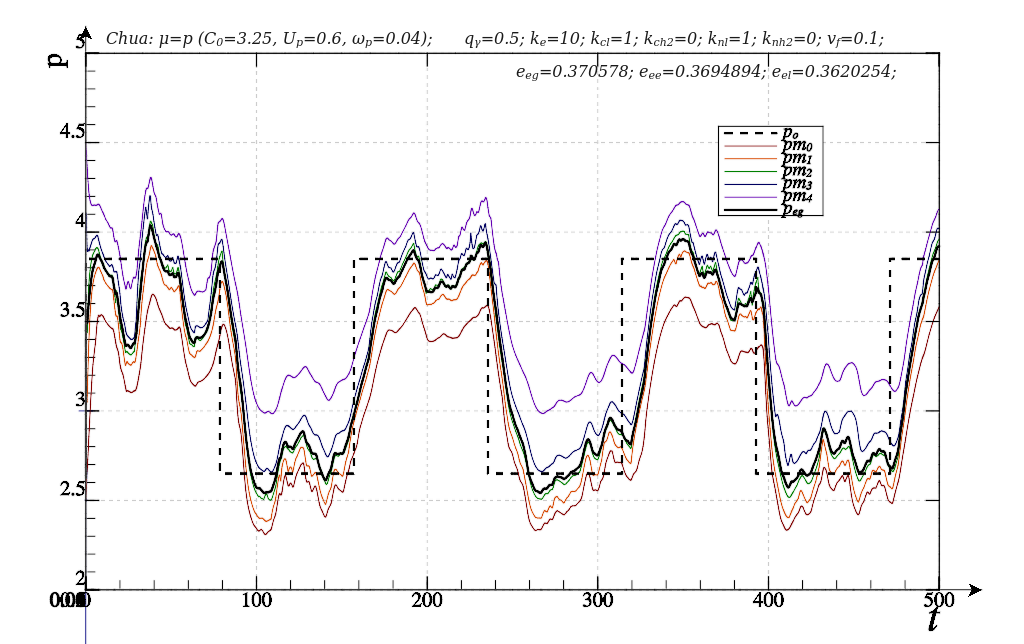
\includegraphics[width=0.49\textwidth]{p/cha/chua/chua_m5p-pl_n_sign.png}
  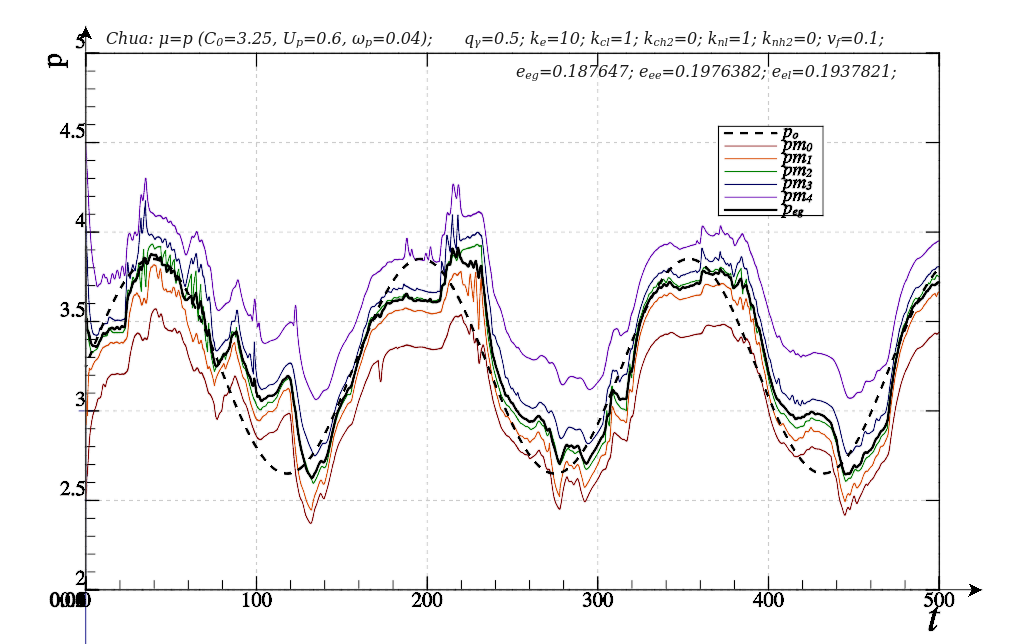
\includegraphics[width=0.49\textwidth]{p/cha/chua/chua_m5p-pl_n_sin.png}
}
\caption{Процесс идентификации параметра $\mu$ системы (\ref{atu:eq:chua2})
  при условиях (\ref{atu:eq:chua_mu_sign}) и (\ref{atu:eq:chua_mu_sin})
}
\label{atu:f:chua_id}
\end{figure}

Для более точной настройки параметров самой системы идентификации
рассмотрим зависимости среднеквадратических ошибок идентификации
от основных параметров системы идентификации.

Одним из важнейших параметров является $q_\gamma$ -- масштаб функции качества.
Зависимости для этого параметра приведены на рис.~\ref{atu:f:chua_e_qgamma}.

\begin{figure}[htb!]
\centerline{
  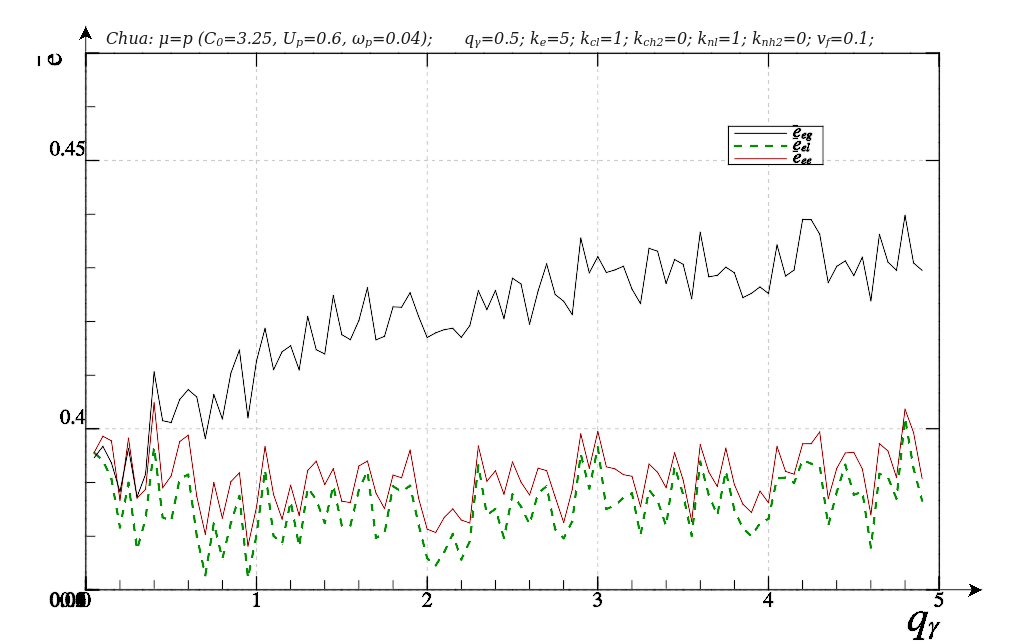
\includegraphics[width=0.49\textwidth]{p/cha/chua/chua_m5p-p_qg_e_sign.png}
  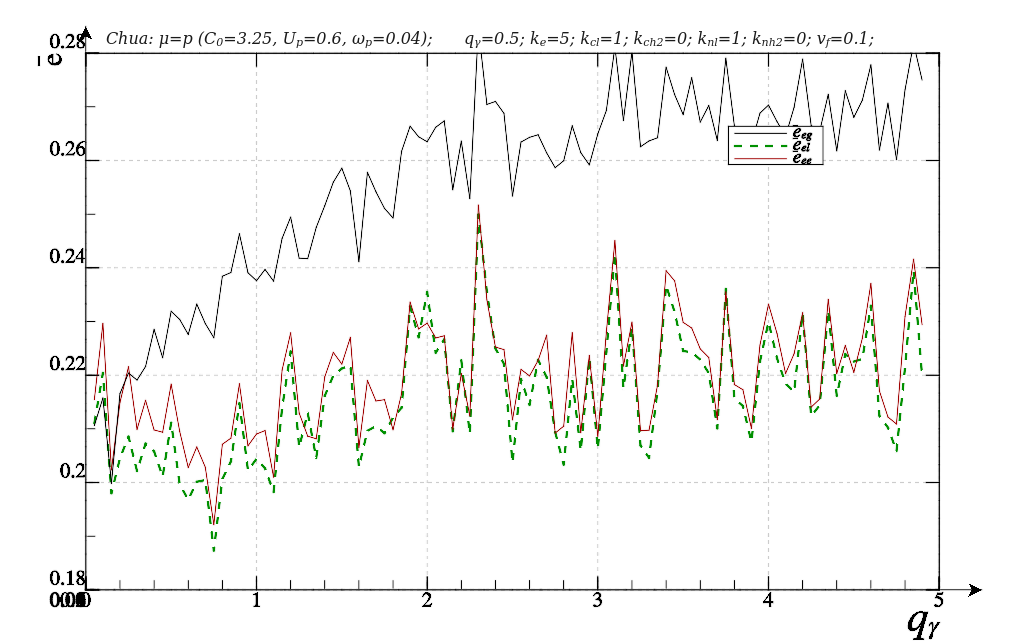
\includegraphics[width=0.49\textwidth]{p/cha/chua/chua_m5p-p_qg_e_sin.png}
}
  \caption{Зависимости  $\bar{e}(q_\gamma)$ для системы (\ref{atu:eq:chua2})
  при условиях (\ref{atu:eq:chua_mu_sign}) и (\ref{atu:eq:chua_mu_sin})
}
\label{atu:f:chua_e_qgamma}
\end{figure}

Явно выраженного экстремума не было обнаружено, что свидетельствует
о сильной робастности метода.

Для проверки корректности выбора величины $a_q$ была построены зависимости
среднеквадратических ошибок идентификации (рис.\ref{atu:f:chua_e_a_q}).


\begin{figure}[htb!]
\centerline{
  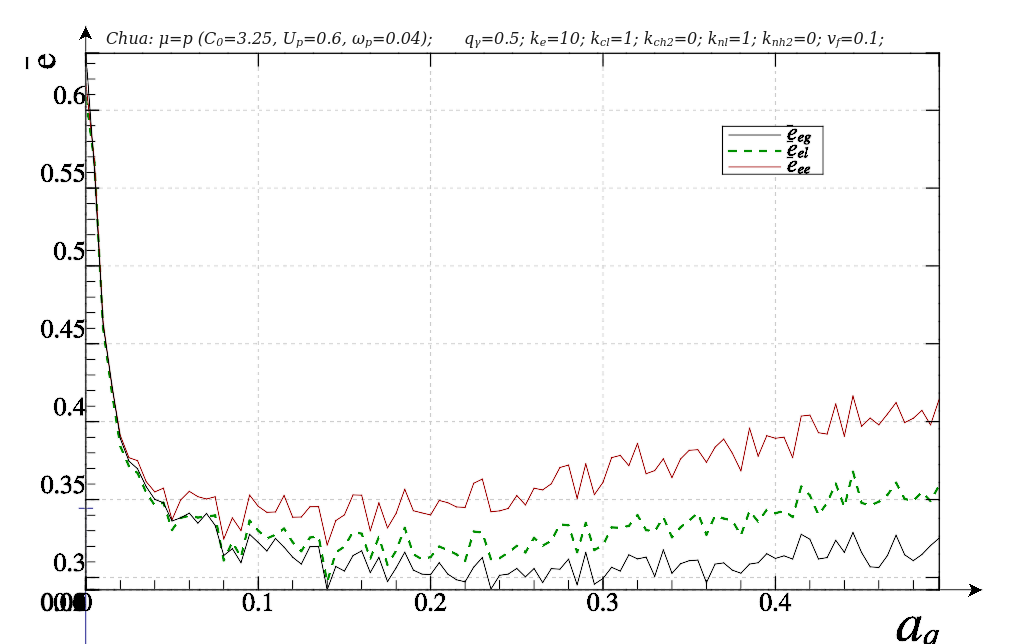
\includegraphics[width=0.49\textwidth]{p/cha/chua/chua_m5p-p_a_q_e_sign.png}
  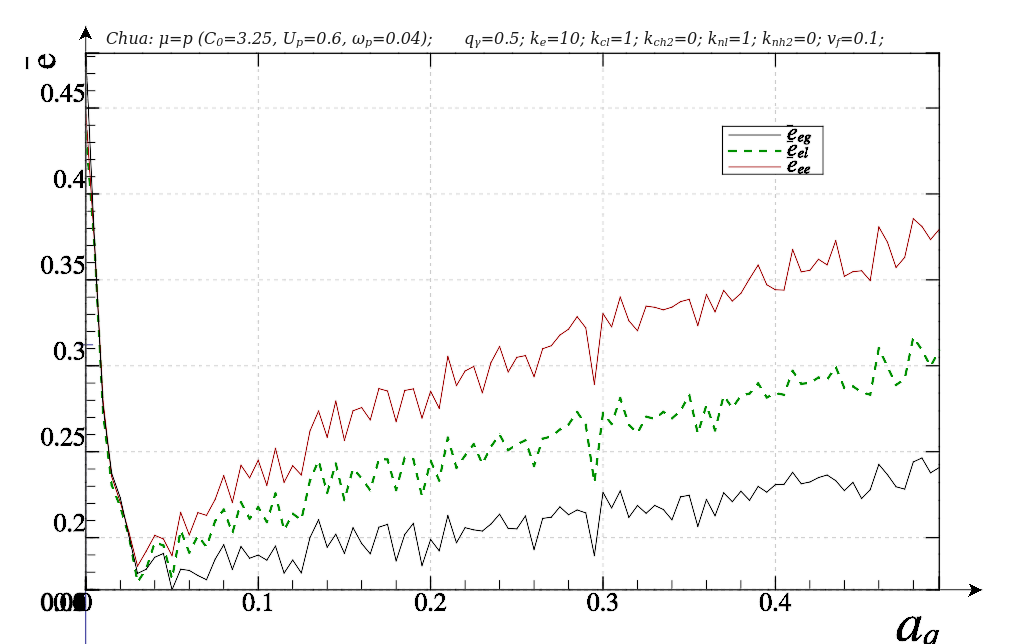
\includegraphics[width=0.49\textwidth]{p/cha/chua/chua_m5p-p_a_q_e_sin.png}
}
  \caption{Зависимости  $\bar{e}(a_q)$ для системы (\ref{atu:eq:chua2})
  при условиях (\ref{atu:eq:chua_mu_sign}) и (\ref{atu:eq:chua_mu_sin})
}
\label{atu:f:chua_e_a_q}
\end{figure}

Как и следовало ожидать, первоначальная оценка ``правильного'' значения величины $a_q$
была сделана достаточно точно. При этом, при синусоидальном изменении параметра объекта
меньшая ошибка идентификации наблюдается при меньших значениях $a_q$, что связано
с тем, в данном случае нет необходимости в слежении за скачкообразно изменяющимся параметром,
и, следовательно, допустимо большее время оценивания. Напротив, в случае (\ref{atu:eq:chua_mu_sign})
увеличение времени оценивания приводит к заметному снижению интегральной точности идентификации.



\FloatBarrier
\subsubsection{Система Рёсслера} % _ROSS_

\LinkRef{
  ross: ASAU-14. ISDMCI-2011, ISDMCI-2012
}

\begin{equation}
\begin{cases}
  \dot{x}  = -y - z  ,  \\
  \dot{y}  = x + a y ,\\
  \dot{z}  = b + z \cdot ( x-c ) .
\end{cases}
\label{atu:eq:rossler}
\end{equation}

Идентифицируемый параметр:
$ c \in [2; 50] $, $c_0=5.88$.

Остальные параметры:
\( a \in (0, 0.35 ) \), $a_0=0.25$,
\(b \in[0;4] \), $b_0=1$.

\begin{figure}[htb!]
\centerline{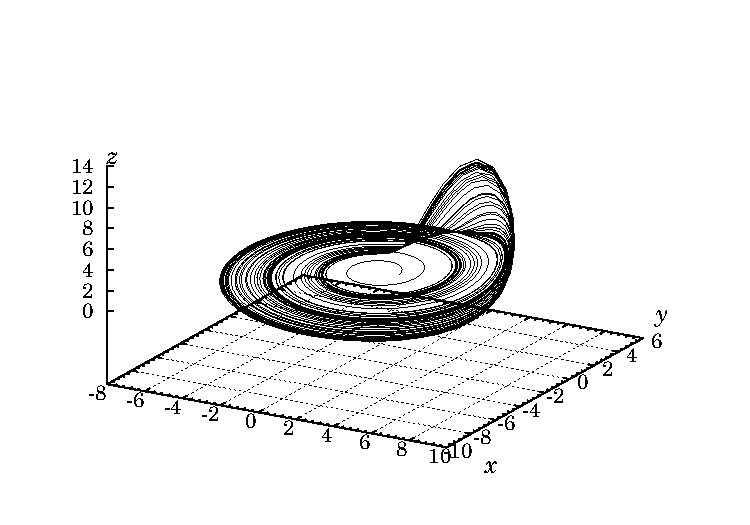
\includegraphics[width=0.6\textwidth]{p/cha/ross_phase3.pdf} }
\caption{Аттрактор системы Рёсслера (\ref{atu:eq:rossler})}
\label{atu:f:ross_phase}
\end{figure}

Критерий
$ z_{\max}$, $ \overline{z} $.



\FloatBarrier
\subsubsection{Система Ван-дер-Поля} % _VDP_

\LinkRef{
  vdp: ASAU-16, 17(alt), ITMM-2011
}

\begin{equation}
 \ddot{x} + \varepsilon (1-x^2)  \dot{x} + \Omega_0^2 x  = u(t) .
\label{atu:eq:vdp}
\end{equation}

\( u(t) = U_{in} \sin ( \omega_{in} t ) \),

Идентифицируемый параметр:
\( \varepsilon \in [1;2]  \)

Остальные параметры:
\(U_{in}=0.3\),
\(\omega_{in}=0.2715\).


\begin{figure}[htb!]
\centerline{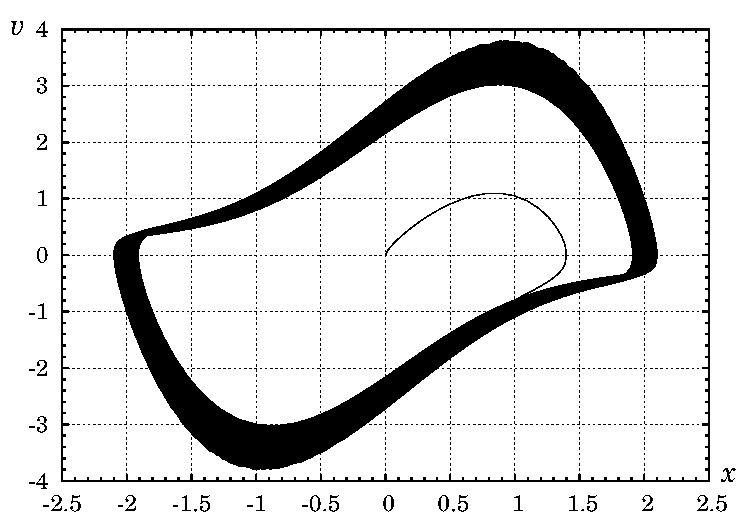
\includegraphics[width=0.5\textwidth]{p/cha/vdp_phase.pdf} }
\caption{Фазовый портрет системы Ван-дер-Поля (\ref{atu:eq:vdp})}
\label{atu:f:vdp_phase}
\end{figure}

Критерий:
$\overline{T}$ + люфт + sign.

Альтернативный критерий:
$\overline{x^2}$


\FloatBarrier
\subsubsection{Генератор Колпитца} % _COLP_

\LinkRef{
  colp: ASAU-21, APIR-2013
}

В  практике   создания   радиоэлектронных   устройств   часто   используются
генераторы сигналов, способные генерировать разнообразные виды  сигналов, в том числе
сложно-периодические и хаотические.
В частности, генератор  Колпитца~[??], в  зависимости   от   условий,   может
генерировать  колебания,  как  близкие  к  гармоническим,  так  и  проявлять
хаотическую  динамику  в  широком  спектральном   диапазоне.   Идентификация
параметров рассматриваемого генератора  необходима,  с  одной  стороны,  для
обеспечения  требуемого  режима  работы.  С  другой  стороны,  информация  о
параметрах системы необходима при проведении  контроля  работоспособности  в
процессе эксплуатации~[??].

На рис.~\ref{atu:f:colp_schem} приставлена одна из электрических схем,
реализующих генератор Колпитца на биполярном транзисторе.
Из множества схем данная была выбрана из-за наличия
одного источника напряжения, и простоты схемотехнической реализации.


\begin{figure}[htb!]
\begin{center}
% vi:syntax=tex

\begin{circuitikz}[line width=0.7]
  \ctikzset{bipoles/thickness=2}
  \def\Top{8.0}
  %
  \draw (3.0,3.0) node[npn](npn) {};
  \draw (2.8,3.0) circle[radius=0.5];
  %\draw (npn.center) circle[radius=0.5];
  %
  \draw (0.0,0.0)
   to[R,l=$R_2$,-*]  (0.0,3.0)
   to[R,l=$R_1$]     (0.0,\Top)
   to[short]         (6.0,\Top)
   to[battery,l=$V_{cc}$] (6.0,0.0)
   -- (0.0,0.0);
  %
  \draw (1.5,0.0) to[C,l=$C_0$,*-*] (1.5,3.0);
  \draw (0.0,3.0) -- (npn.base);
  \draw (3.0,0.0) to[vR,l=$R_e$,*-*] (3.0,2.0)
   to[short] (npn.emitter);
  \draw (npn.collector)
   to[L,l=$L$,i<=$I_L$] (3.0,6.0)
   to[R,l=$R_c$] (3.0,\Top);
  %
  \draw (4.5,0.0) to[C,l=$C_2$,v=$V_2$,*-*] (4.5,2.0);
  \draw (4.5,2.0) -- (3.0,2.0);
  \draw (4.5,2.0) to[C,l=$C_1$,v=$V_1$]     (4.5,4.0);
  \draw (4.5,4.0) -- (3.0,4.0);
  \filldraw (3.0,4.0) circle[radius=0.05];
\end{circuitikz}



%\begin{tikzpicture}[circuit ee IEC,very thick,circuit symbol unit=2.5mm]
%%\tikzset{circuit declare symbol=transistor}
%%\tikzset{set transistor graphic=transistor IEC graphic}
%  \node (R2)    at (0.0,0.0) [elelem,point up,resistor={info = $R_2$}] {};
%  \node (pR1R2) at (0.0,1.5) [contact] {};
%  \node (R1)    at (0.0,3.0) [elelem,point up,resistor={info = $R_1$}] {};
%  %
%  \node (C0)    at (1.5,0.0) [point up,elelem,capacitor={info = $C_0$}] {};
%  \node (pR2C0) at (1.5,1.5) [contact] {};
%  %
%  \node (Re)    at (3.0,0.0) [elelem,point up,resistor={adjustable,info = $R_e$}] {};
%  %\node (Q1)    at (3.0,1.5) [elelem,point right,transistor] {};
%  \node (L)     at (3.0,3.0) [elelem,point up,inductor={info = $L$}] {};
%  \node (Rc)    at (3.0,4.5) [elelem,point up,resistor={info = $R_c$}] {};
%  %
%  \node (C2)    at (4.5,0.0) [point up,elelem,capacitor={info = $C_2$}] {};
%  \node (C1)    at (4.5,3.0) [point up,elelem,capacitor={info = $C_1$}] {};
%  %
%  \node (Bat)   at (6.0,0.0) [point up,elelem,battery={info = $Vcc$}] {};
%\end{tikzpicture}


\end{center}
\caption{Электрическая схема генератора Колпитца на биполярном транзисторе}
\label{atu:f:colp_schem}
\end{figure}

При создании модели генератора Колпитца систему уравнений можно
заранее упростить, если заметить, что
делитель на резисторах
$\mathrm{R}_1$, $\mathrm{R}_2$,
вместе с конденсатором
$\mathrm{C}_0$ обеспечивают
постоянство потенциала базы
$V_b = V_{CC} \frac{R_1}{R_1+R_2}$,
поэтому из дальнейшего рассмотрения данные элементы следует
исключить.

Рассмотрев процессы заряда конденсаторов и изменение тока через
катушку идуктивности, получим следующую систему уравнений:

\begin{equation}
\label{atu:eq:colp_phys}
\begin{dcases}
  C_1 \frac{dV_{1}}{dt}  = I_L - I_{CE} , \\
  L   \frac{dI_L}{dt}    = V_{CC} - V_{1} - V_{2} - I_L R_C , \\
  C_2 \frac{dV_{2}}{dt}  = I_L - \frac{V_{2}}{R_e}.
\end{dcases}
\end{equation}


\noindent
где
$V_{CC} $ -- напряжение питания,
$V_1,$ $V_2$ -- разность потенциалов между выводами конденсаторов
$\mathrm{C}_1$ и $\mathrm{C}_2$ соответственно,
$I_L$, $I_{CE}$ -- токи катушки индуктивности и транзистора (коллектор-эмиттер).

Перейдём к безразмерным величинам.
При переходе к безразмерному виду следует определить,
какие физические параметры определяют безразмерные величины.
Это потребуется для синтеза критерия идентификации.
Для упрощения рассмотрения, не снижая общности,
будем считать $C_1 = C_2 = C$.

Прежде всего, воспользуемся тем, что система содержит только один
активный нелинейный компонент -- транзистор.
Следовательно, именно этот элемент определяет
масштаб по напряжению. В простейшей модели транзистора
такой масштабной величиной может служить
$V_{je}$ -- падение напряжения на переходе база-эмиттер
в активном режиме. Следовательно, все разности потенциалов в схеме можно нормировать
на эту величину.

Динамические свойства (в т.ч. условия начала генерации и перехода в хаотический режим) определяются
соотношением активных и реактивных свойств системы. При этом величина
$ \rho = \sqrt{L/C} $ имеет размерность сопротивления
и определяет реактивное сопротивление. Эту величину можно использовать
для обезразмеривания активных сопротивлений.

Для приведения токов к безразмерному виду, с учётом уже выбранных величин,
следует использовать величину $ V_{je} / \rho$.


Исходя из всего вышеперечисленного, обозначим:

\[
  x = \frac{V_{1}}{V_{je}} ; \quad
  y = \frac{\rho I_L}{V_{je}} ; \quad
  z = \frac{V_{2}}{V_{je}}, \quad
  i_{ce} = \frac{\rho I_{ce}}{V_{je}}, \quad
  c = \frac{V_{CC}}{V_{je}}, \quad
  e = \frac{V_{b}}{V_{je}}.
\]
\[
  b = \frac{R_c}{\rho}; \quad
  d = \frac{\rho}{R_e}. % sic!
\]

Система уравнений принимает вид:


\begin{equation}
\label{atu:eq:colp_phys2}
\begin{dcases}
  \dfrac{d x}{dt}  = \dfrac{1}{\rho C}  y - \dfrac{1}{\rho C} i_{ce} , \\
  \dfrac{d y}{dt}  = \dfrac{\rho}{L} c    - \dfrac{\rho}{L} r_c y - \dfrac{\rho}{L} x- \dfrac{\rho}{L} z, \\
  \dfrac{d_z}{dt}  = \dfrac{1}{\rho C}  y - \dfrac{1}{\rho C} \dfrac{1}{r_e} z.
\end{dcases}
\end{equation}

Общий множитель $ \frac{1}{\rho C} = \frac{\rho}{L} = \sqrt{\frac{1}{LC}} $ в правых частях уравнений
естественным образом задаёт масштаб по времени.
Это подчёркивает, что частотные характеристики рассматриваемого генератора,
в отличие, например, от релаксационного,
определяются ёмкостью и индуктивностью,
поэтому масштаб времени задаём так:
$ T_s = \sqrt{L C} $.
Тогда безразмерное время $t_s$
и соответствующие производные
будут определены таким образом:

\[
  t_s = \frac{t}{T_s}; \quad
  dt = T_s dt_s; \quad
  \frac{d}{dt} = \frac{1}{T_s} \frac{d}{dt_s}; \quad
  \frac{dx}{dt_s} \equiv \dot{x} = T_s \frac{dx}{dt} .
\]

Поведение величины $I_{ce}$ достаточно хорошо описывает модель
Эберса-Молла~[Хоровиц]:

\begin{equation}
  I_c = I_s \left( \exp\frac{V_{be}}U_t{} - 1 \right),
  \label{atu:eq:ebers-moll}
\end{equation}

\noindent
где
$I_s$ -- ток насыщения (паспортная или определяемая экспериментально величина),
$U_t=kT/q$,
$q = \SI{1.6e-19}{\coulomb}$ -- заряд электрона,
$k = \SI{1.38e-24}{\joule/\kelvin}$ -- постоянная Больцмана.
Необходимо учесть, что в режиме отсечки ($V_b < V_e$) ток коллектора пренебрежимо мал,
а в режиме насыщения определяется другими элементами схемы.
Существуют и более сложные модели, например,
программы для моделирования электронных схем часто используют так называемую SPICE модель.

К сожалению, при моделировании генератора Колпитца в литературе,
посвящённой хаотической динамике, используют
простейшую модель транзистора, считая, что переход
база-эмиттер открывается при $V_{BE} = V_{je}$, $ I_c \gg I_b$,
а ток коллектора

\begin{equation}
I_c =
  \begin{cases}
    \alpha ( V_b - V_e - V_{je} ), & V_b - V_e > V_{je} \\
    0                              & \text{otherwise}.
  \end{cases}
  \label{atu:eq:bjt_libear_model}
\end{equation}



С учётом всего вышеизложенного получаем следующую систему уравнений:

\begin{equation}
\label{atu:eq:colp}
\begin{cases}
  \dot{x} = y - a F(z), \\
  \dot{y} = c - x - by - z, \\
  \dot{z} = y - d z.
\end{cases}
\end{equation}

При этом параметр $b$ характеризует соотношение
активного и реактивного сопротивления,
и, следовательно, режима работы генератора.
Величиной этого параметра проще всего управлять,
изменяя $R_c$.
Поставленной задачей будем считать идентификацию
данного параметра.

При физическом моделировании в рамках данной работы использовались следующие
элементы с соответствующими параметрами:

\[
  V_{cc} = \SI{12.06}{\volt},          \;
  R_1 = R_2 = \SI{2.2}{\kilo\ohm},     \;
  R_e = \SI{430}{\ohm},                \;
  C_1 = C_2 = \SI{1.03}{\micro\farad}, \;
  L = \SI{6.22}{\milli\henry},         \;
  T = \SI{305}{\kelvin},
\]

\[
  \text{Q: 2N2222A}, \quad
  h_{fe}=285, \quad
  V_f = \SI{0.677}{\volt}, \quad
  I_s = \SI{9.61e-14}{\ampere}, \quad
  \alpha \approx 1.
\]

Тогда безразмерные коэффициенты:
\[
 a = 77,     \quad
 c = 18.08,  \quad
 d = 0.19,   \quad
 e = 9.07.
\]

\[
F(z) =
\begin{cases}{l}
  e-1-z, & z \le e-1  \\
  0,     & z  >  e-1
\end{cases}.
\]


Диапазон изменения идентифицируемого параметра
$b \in [ 0.02; 4.2 ]$
определяется, с одной стороны, собственным сопротивлением катушки индуктивности,
с другой -- срывом генерации.


На рис.~\ref{atu:f:colp_real_xzz}--\ref{atu:f:colp_model_f} предствлены как результаты реального эксперимента,
так и данные, полученные в результате численного моделирования динамики системы (\ref{atu:eq:colp}).
Представлены проекции аттракторов но плоскость $(x+z,z)$ (естественный вид для оциллографа),
трёхмерный вид аттракторов, и спектры.
На каждом рисунке представлено три режима: обычный, момент первого удвоения периода и хаотический режим.


\begin{figure}[htb!]
 \centerline{
   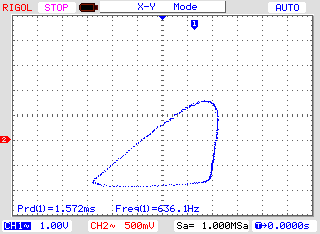
\includegraphics[width=0.32\textwidth]{p/cha/colp/colp_m1_vv.png}
   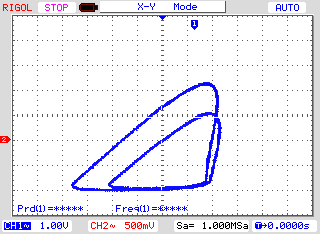
\includegraphics[width=0.32\textwidth]{p/cha/colp/colp_m2_vv.png}
   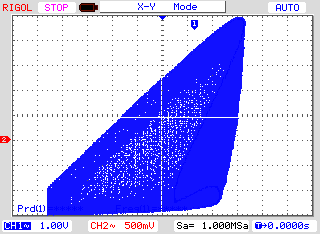
\includegraphics[width=0.32\textwidth]{p/cha/colp/colp_m3_vv_ac.png}
 }
  \caption{Проекции аттракторов реальной системы Колпитца на плоскость $(x+z,z)$
  для трёх режимов}
  \label{atu:f:colp_real_xzz}
\end{figure}

\begin{figure}[htb!]
 \centerline{
   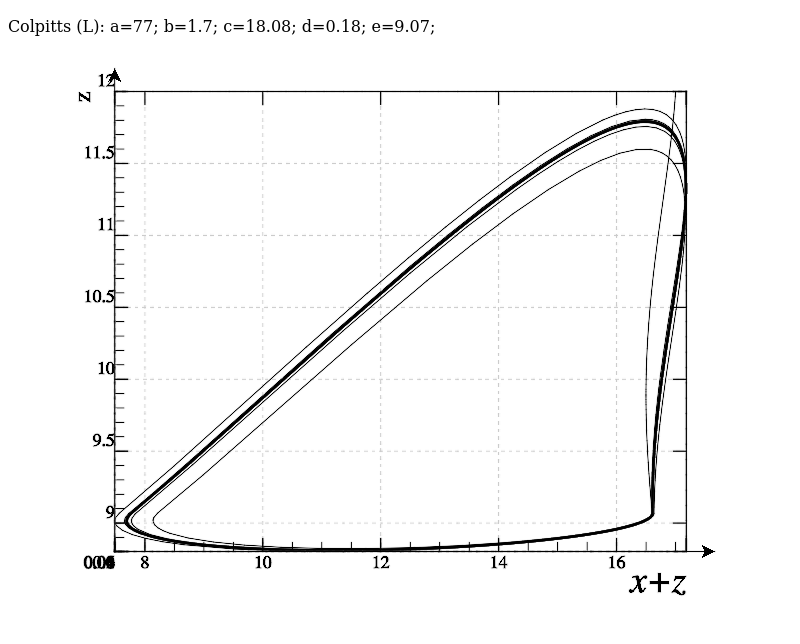
\includegraphics[width=0.32\textwidth]{p/cha/colp/colp_0-p_z_xpz_b=1x70.png}
   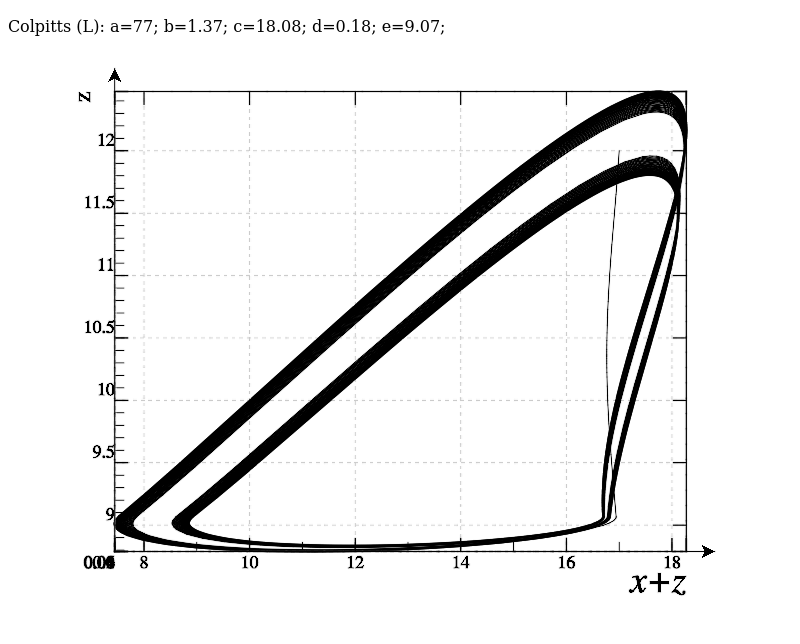
\includegraphics[width=0.32\textwidth]{p/cha/colp/colp_0-p_z_xpz_b=1x37.png}
   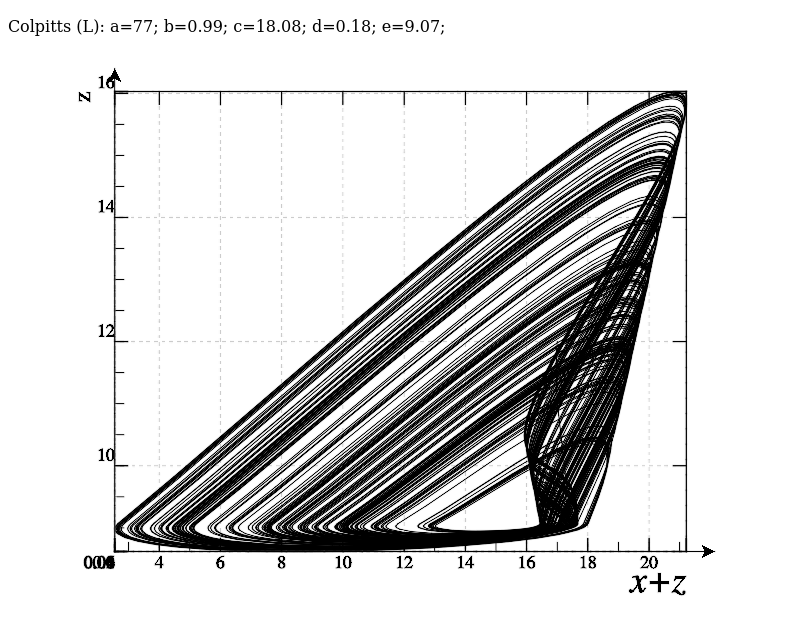
\includegraphics[width=0.32\textwidth]{p/cha/colp/colp_0-p_z_xpz_b=0x99.png}
 }
  \caption{Проекции аттракторов модели (\ref{atu:eq:colp}) системы Колпитца на плоскость $(x+z,z)$
  для трёх режимов}
  \label{atu:f:colp_model_xzz}
\end{figure}


\begin{figure}[htb!]
 \centerline{
   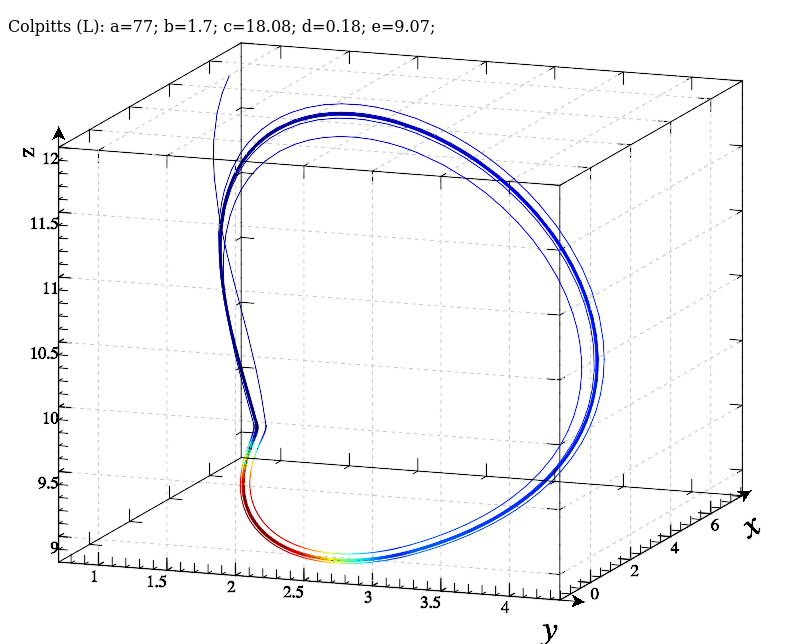
\includegraphics[width=0.32\textwidth]{p/cha/colp/colp_0-p_xyz_b=1x70.png}
   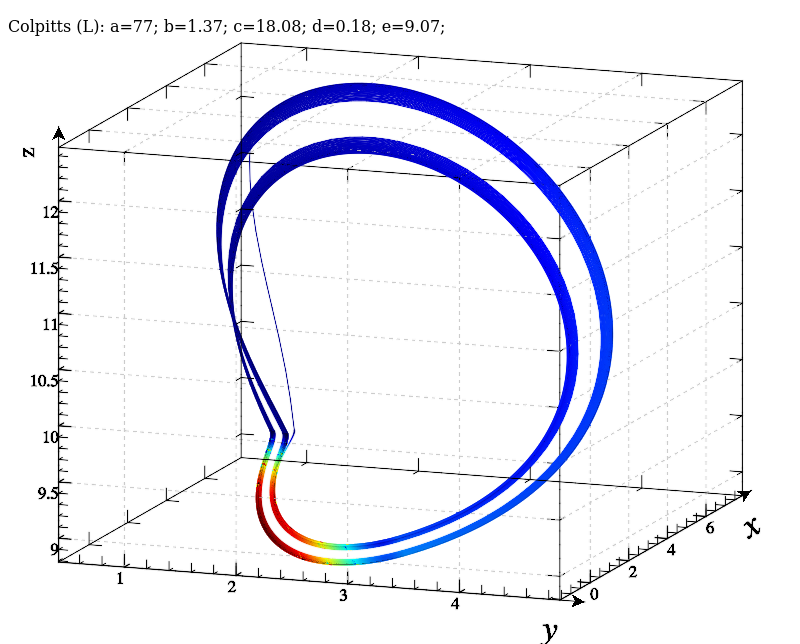
\includegraphics[width=0.32\textwidth]{p/cha/colp/colp_0-p_xyz_b=1x37.png}
   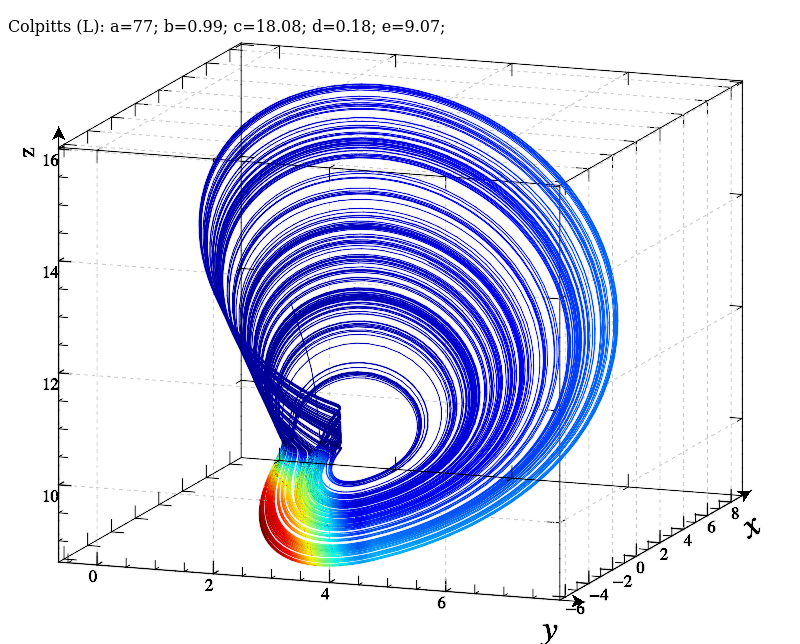
\includegraphics[width=0.32\textwidth]{p/cha/colp/colp_0-p_xyz_b=0x99.png}
 }
  \caption{Аттрактороы модели (\ref{atu:eq:colp}) системы Колпитца для трёх режимов}
  \label{atu:f:colp_model_xyz}
\end{figure}

\begin{figure}[htb!]
 \centerline{
   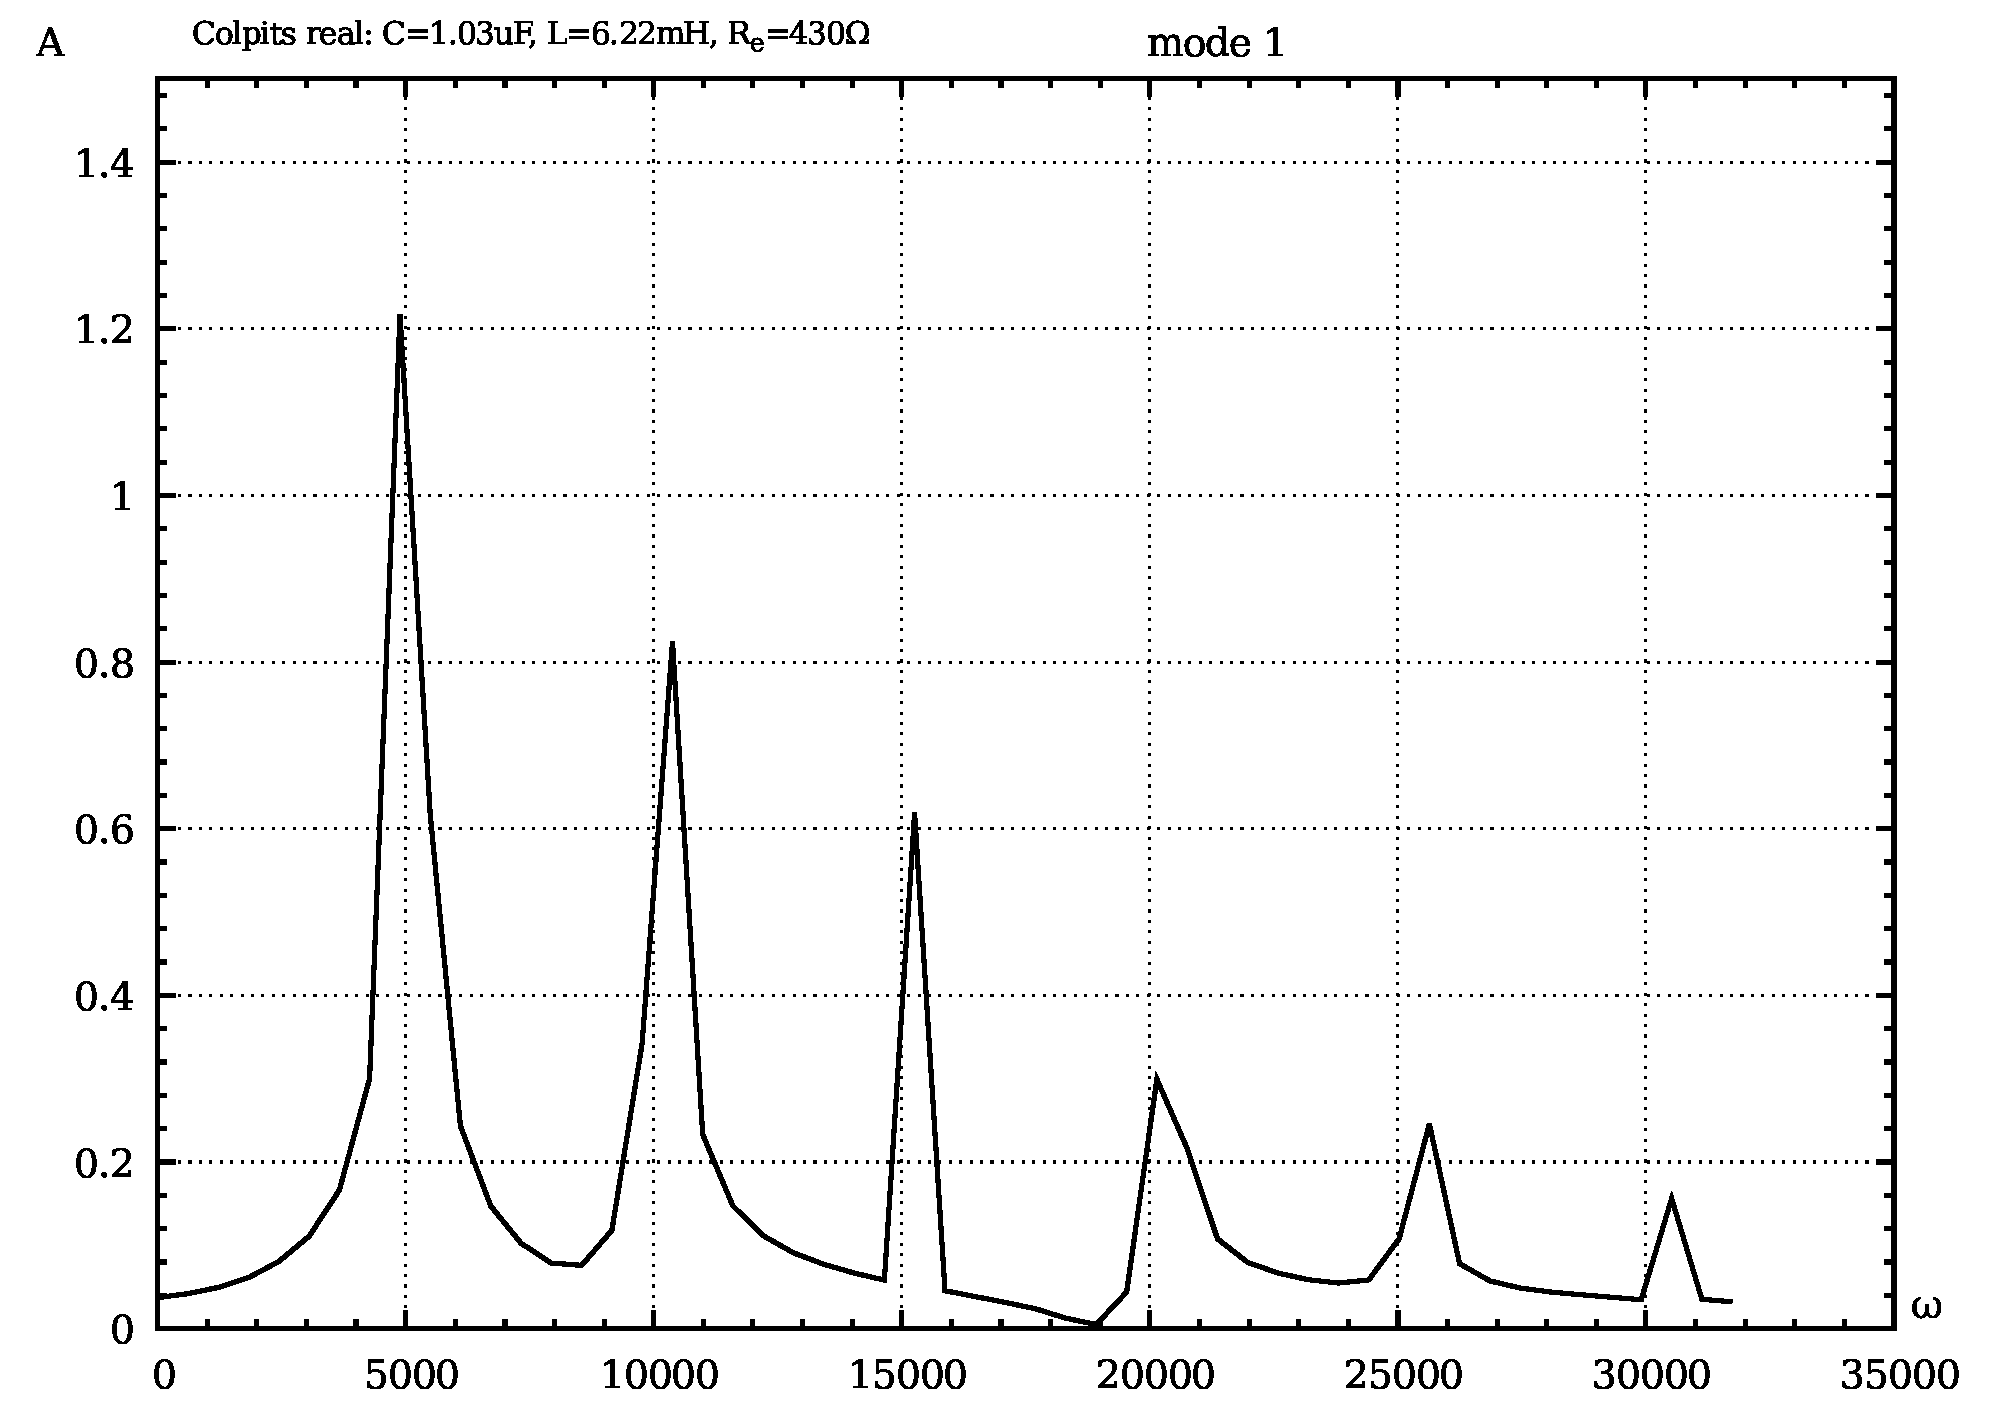
\includegraphics[width=0.32\textwidth]{p/cha/colp/colp_m1_f.png}
   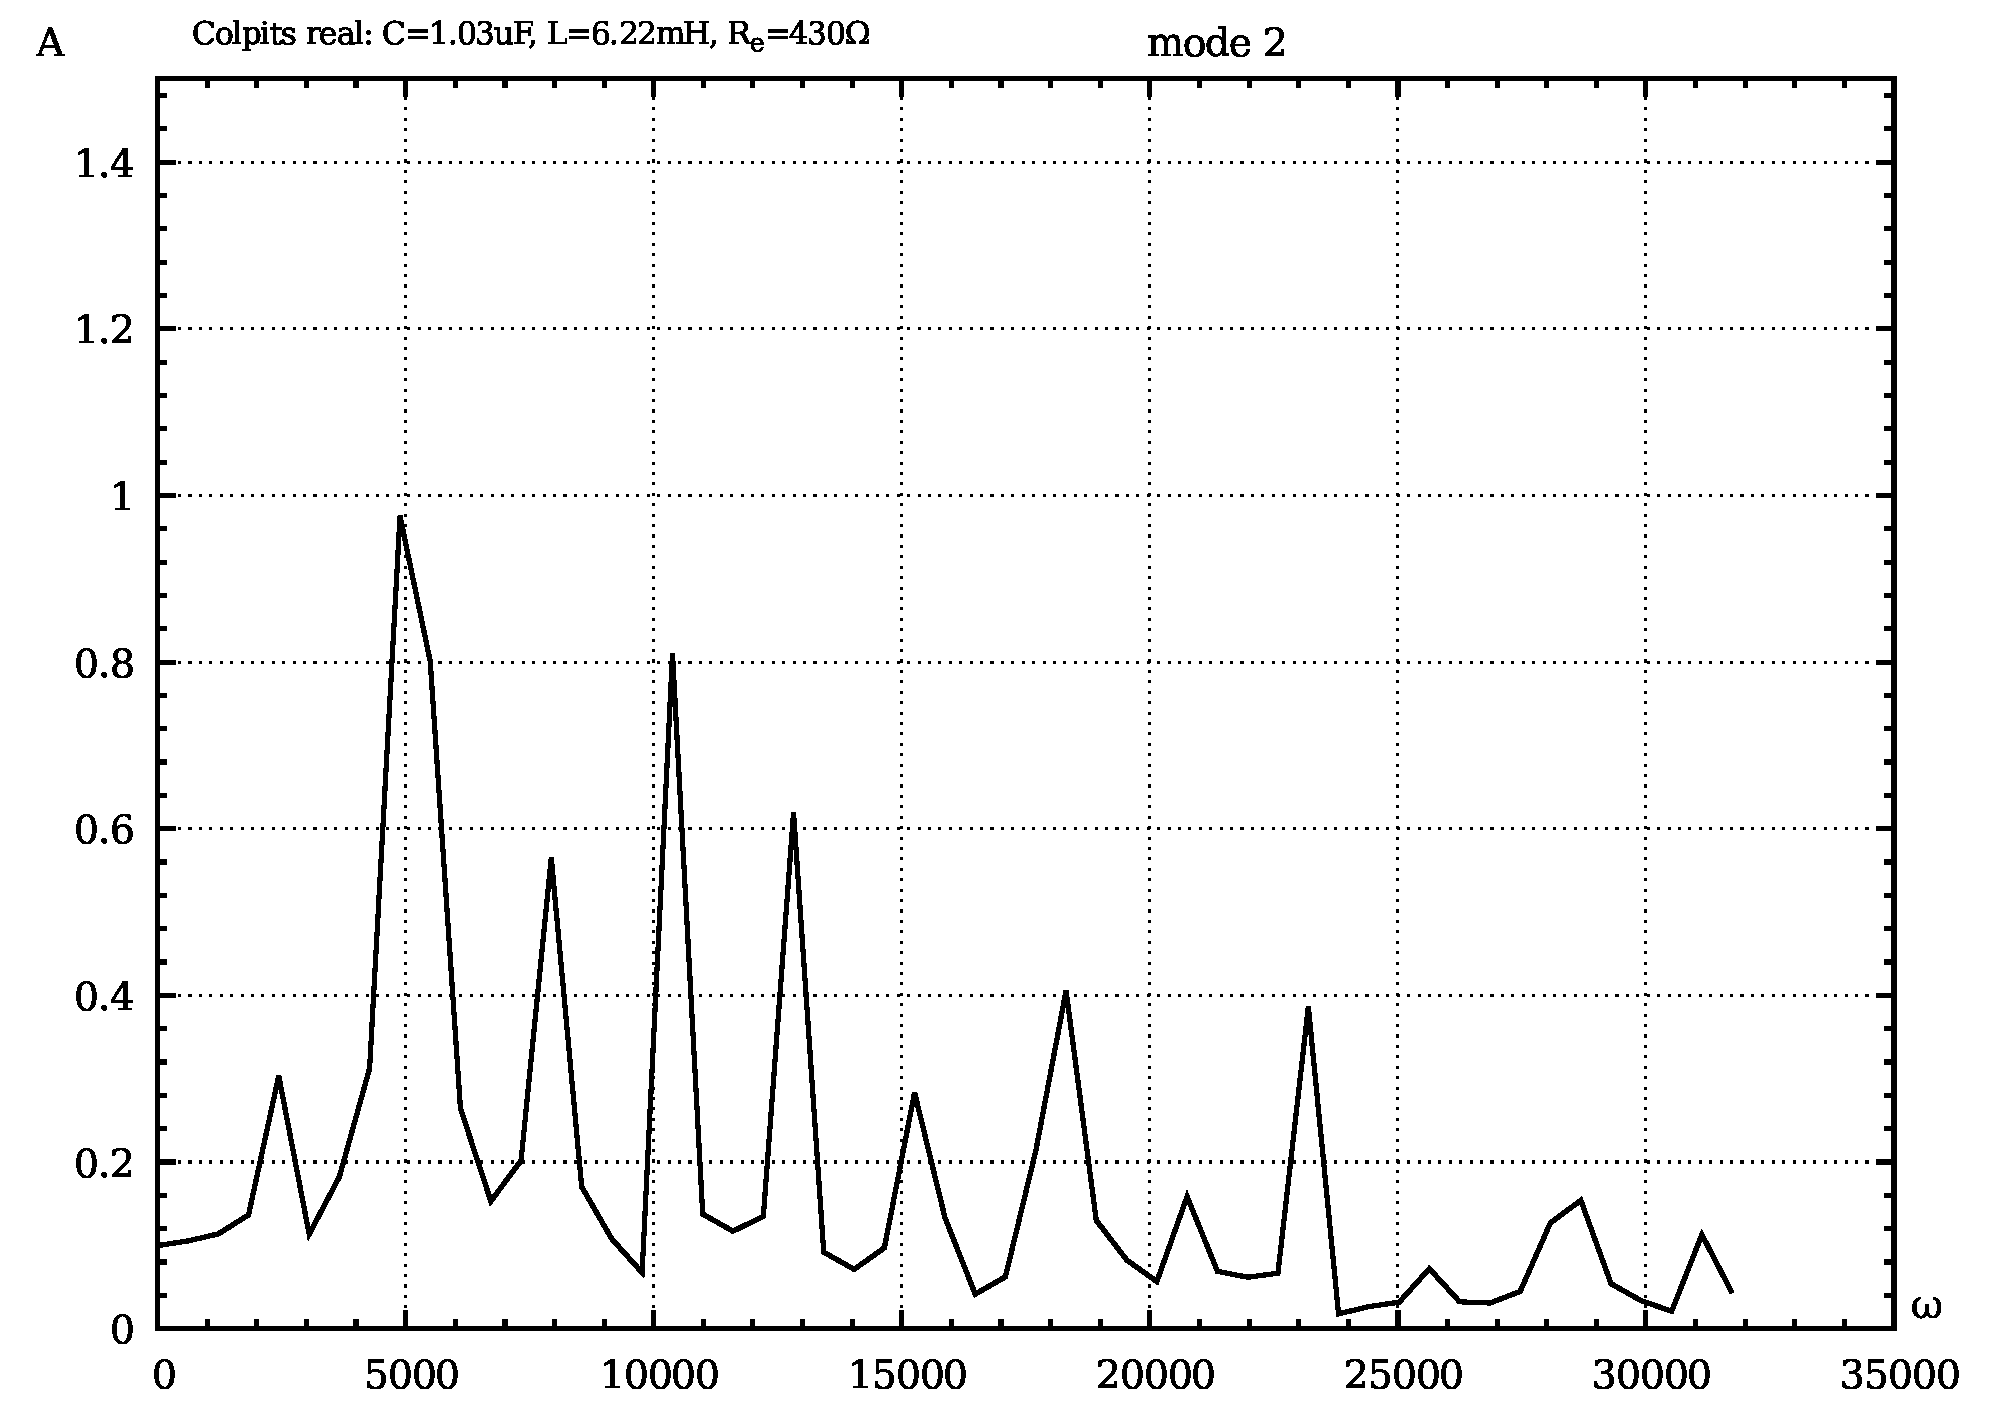
\includegraphics[width=0.32\textwidth]{p/cha/colp/colp_m2_f.png}
   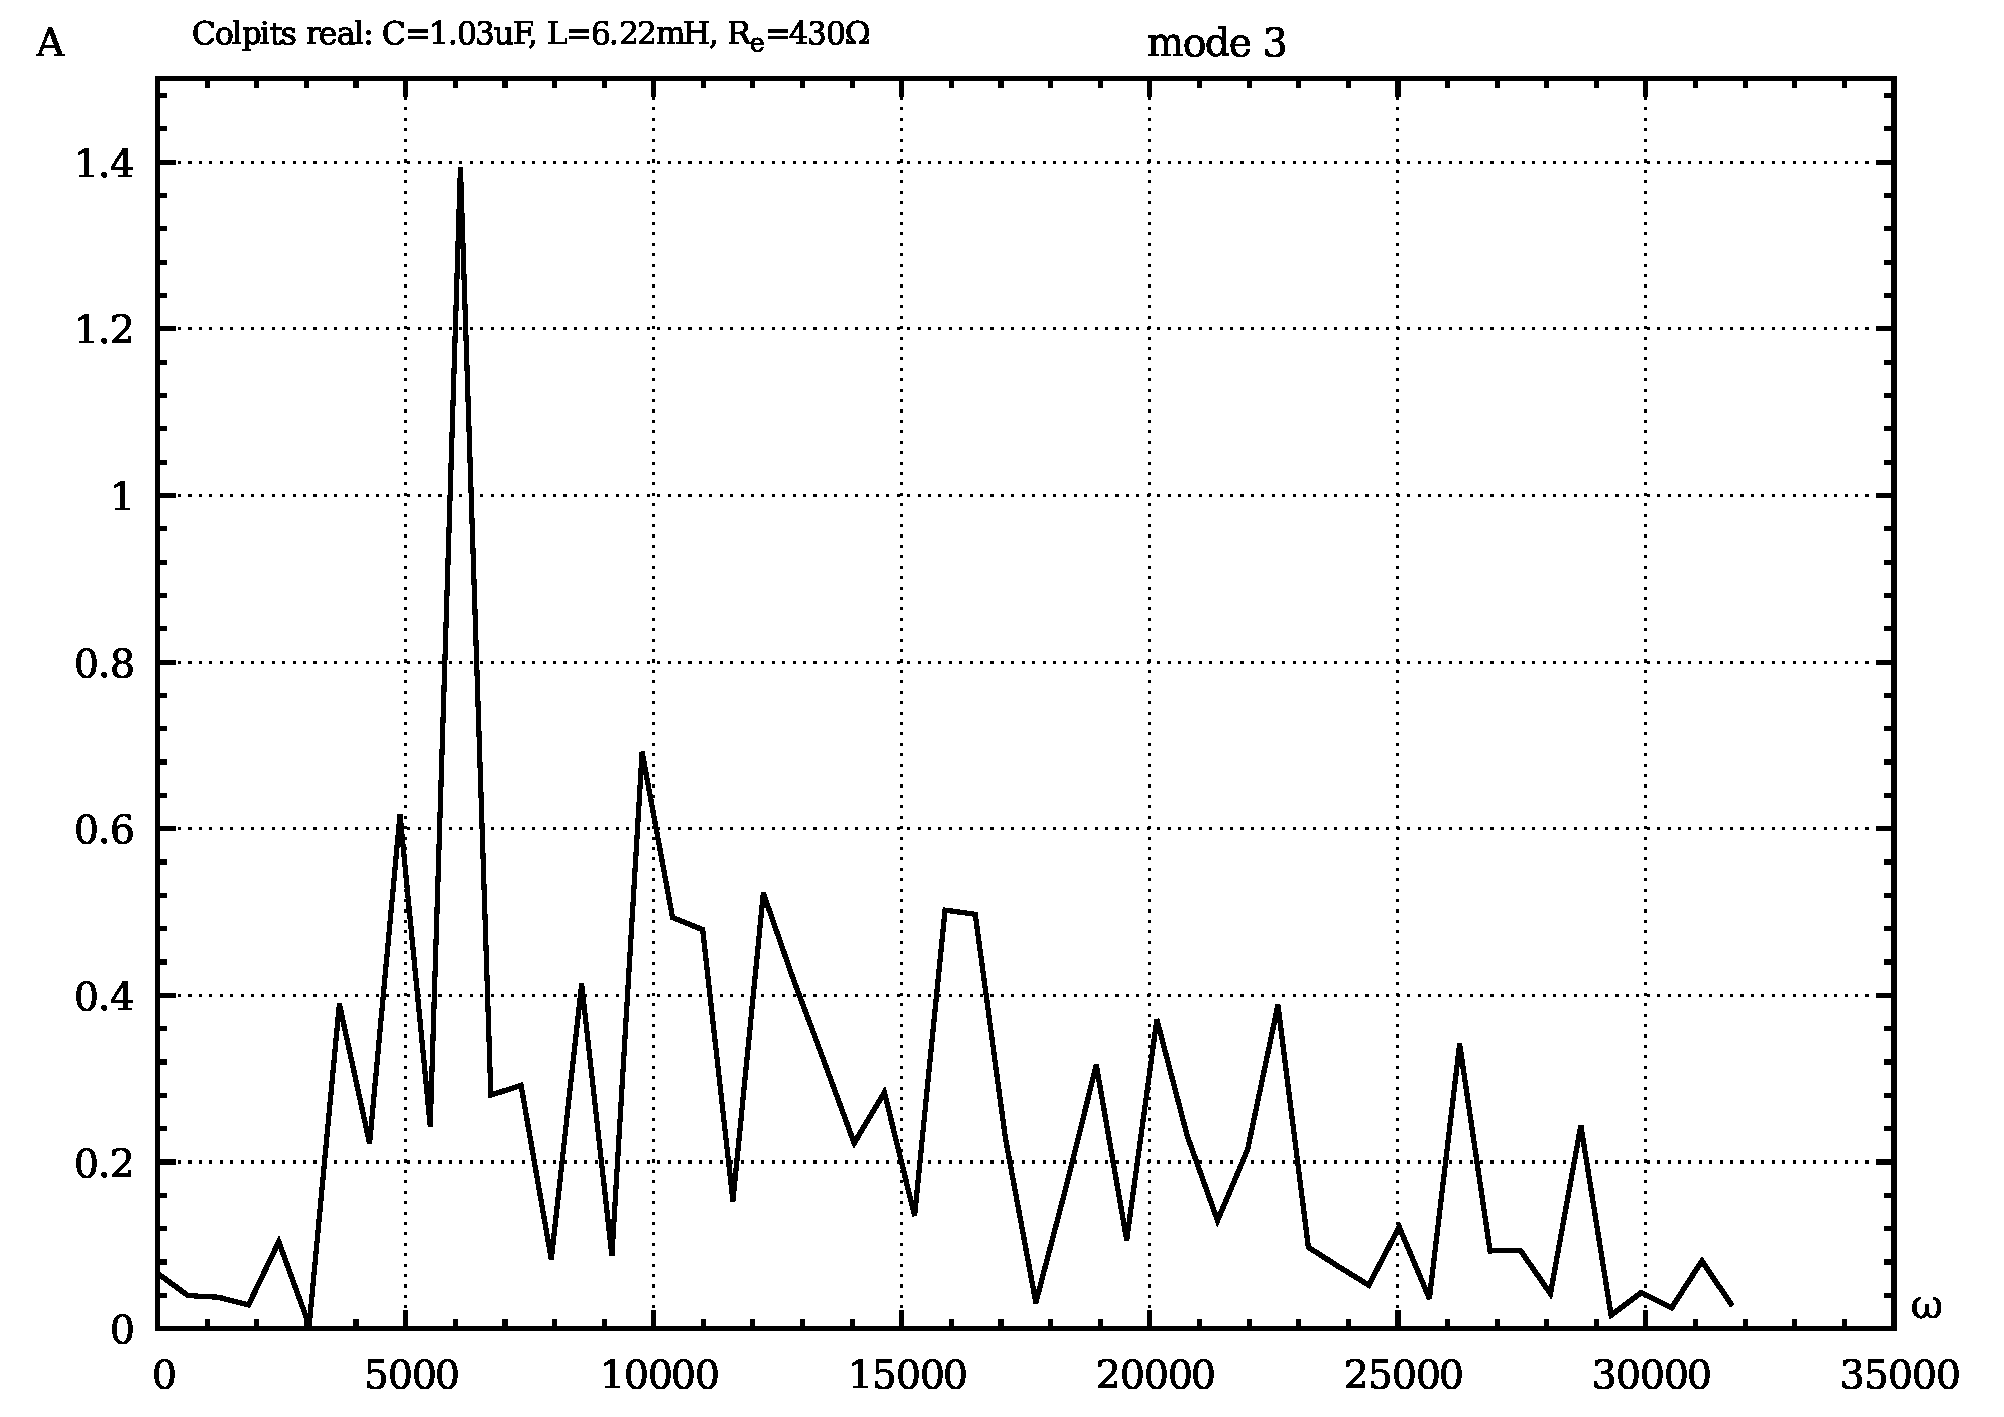
\includegraphics[width=0.32\textwidth]{p/cha/colp/colp_m3_f.png}
 }
  \caption{Спектры реальной системы Колпитца  для трёх режимов}
  \label{atu:f:colp_real_f}
\end{figure}

\begin{figure}[htb!]
 \centerline{
   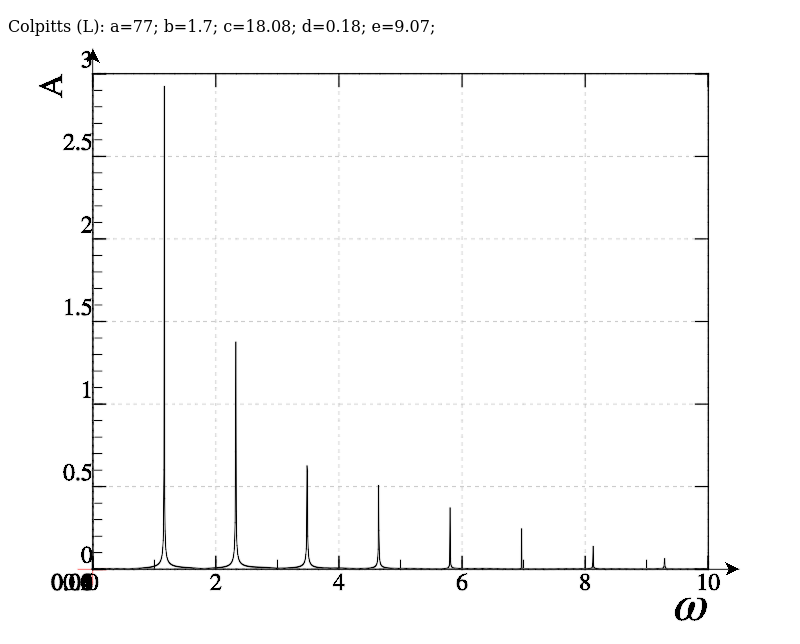
\includegraphics[width=0.32\textwidth]{p/cha/colp/colp_f-p_f_b=1x70.png}
   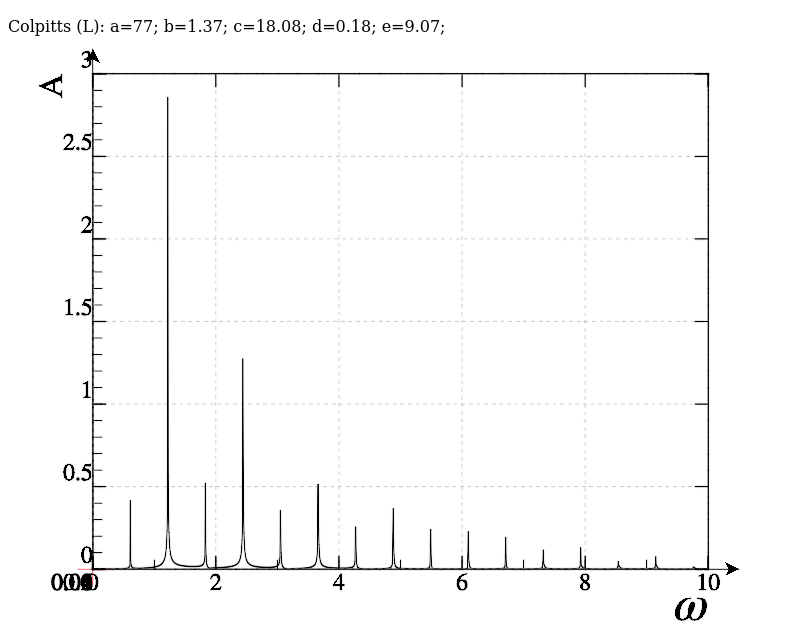
\includegraphics[width=0.32\textwidth]{p/cha/colp/colp_f-p_f_b=1x37.png}
   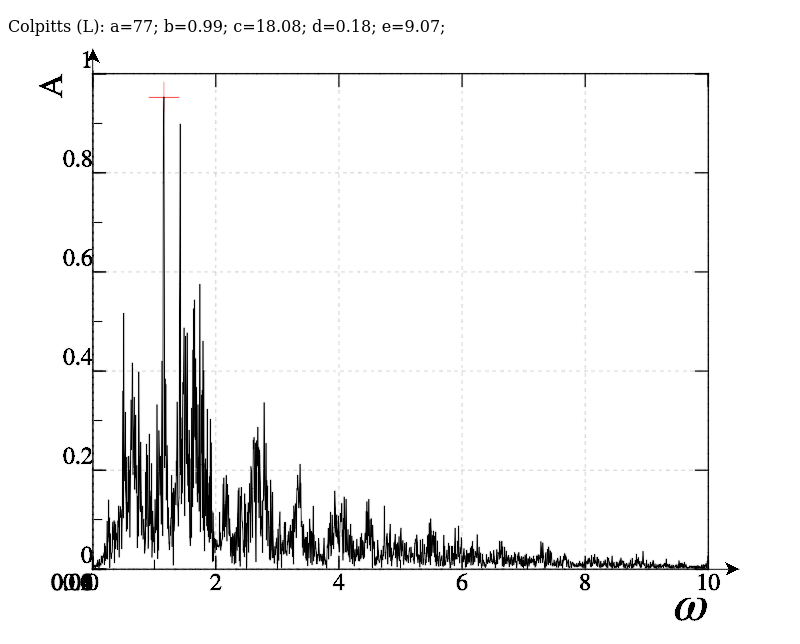
\includegraphics[width=0.32\textwidth]{p/cha/colp/colp_f-p_f_b=0x99.png}
 }
  \caption{Спектры модели (\ref{atu:eq:colp}) системы Колпитца для трёх режимов}
  \label{atu:f:colp_model_f}
\end{figure}

Сравнение результатов физического и численного моделирования позволяет сделать вывод
о качественном подобии поведения реальной системы и модели.
Тем не менее, величины параметра $b$, при которых получены
рассматриваемые режимы, совпадают недостаточно точно.
Для реальной системы значения параметра: $b = 1.06, \; 0.94, \; 0.90 $,
а для модели: $b = 1.70, \; 1.34, \; 0.99 $.
Скорее всего, это связано с грубостью модели (\ref{atu:eq:bjt_libear_model}) транзистора,
и требует дальнейшего исследования.
К сожалению, ограниченный набор данных, получаемых с осциллографа (8192 отсчёта) не позволяют
получить достаточно подробный спектр реальной системы.

Для определения критерия рассмотрим зависимости
$q_{*}(\mu) $, полученные путём моделирования
для системы Колпитца (рис.~\ref{atu:f:colp_q}).
При этом следует учесть, что наиболее просто измерямыми величинами являются $x$ и $z$,
Соответствующие напряжениям $V_1$ и $V_2$.
Первый набор зависимостей даёт два основных кандидата -- $q_{x^2}$ и $q_{z^2}$.
При этом первый из них показывает более равномерную зависимость.
С другой стороны, при большинство из рассморенных зависимостей имею явно
выраженный гиперболический характер, особенно при малых значениях $b$.
Следовательно, в сприсок кандидатов следует добавить $q_{x^{-2}} $ и $q_{z^{-2}}$.

\begin{figure}[htb!]
\centerline{
  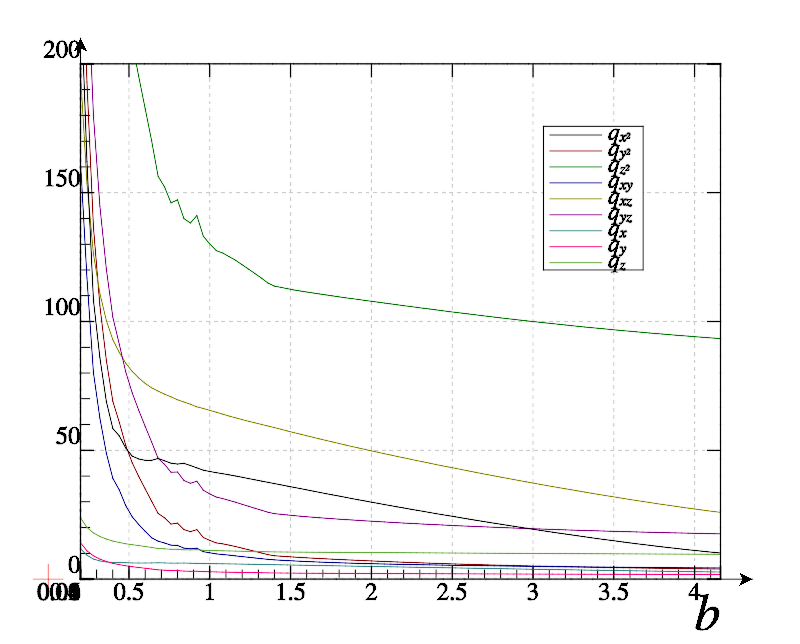
\includegraphics[width=0.49\textwidth]{p/cha/colp/colp_p-p_b_e.png}
  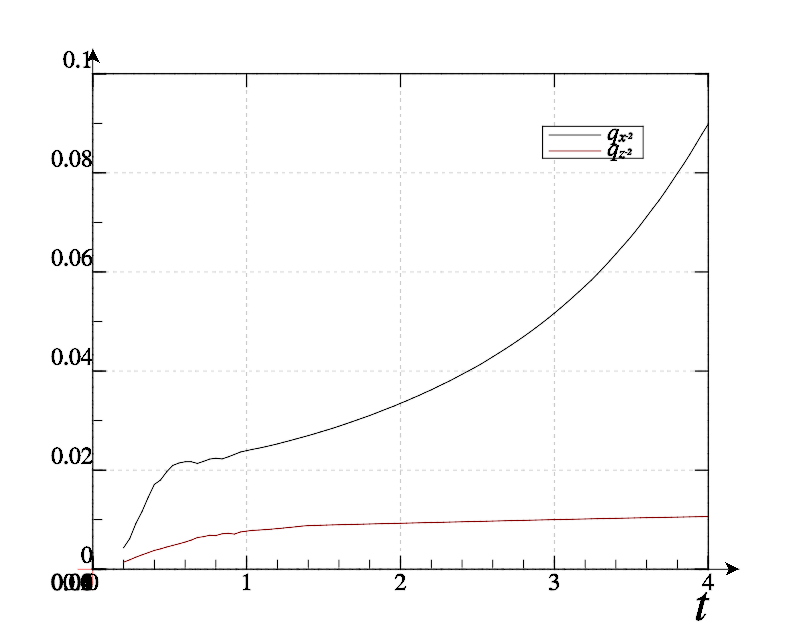
\includegraphics[width=0.49\textwidth]{p/cha/colp/colp_p-p_b_1ex2.png}
}
  \caption{Зависимости $q_{*}(b) $ для системы Колпитца (\ref{atu:eq:colp})}
\label{atu:f:colp_q}
\end{figure}

Из графиков очевидно, что
обратные зависимости не дают заметного выигрыша, поэтому выберем
величину $ q_{x^2}(b) $ в качестве критерия.

В качестве системы идентификации использовалась система с 5 поисковыми агентами и
двумя неподвижными моделями. Аналогично предыдущим системам,
для исследования динамических свойств системы идентификации
параметр $b_o$ так:

\begin{equation}
 b_o(t) = p_0 + U_p \sign \sin( \omega_p t ),
  \label{atu:eq:colp_b_sign}
\end{equation}

\begin{equation}
 b_o(t) = p_0 + U_p \sin( \omega_p t ).
  \label{atu:eq:colp_b_sin}
\end{equation}

Динамика процессов идентификации для системы Колпитца представлена на рис.~\ref{atu:f:colp_id}.

\begin{figure}[htb!]
\centerline{
  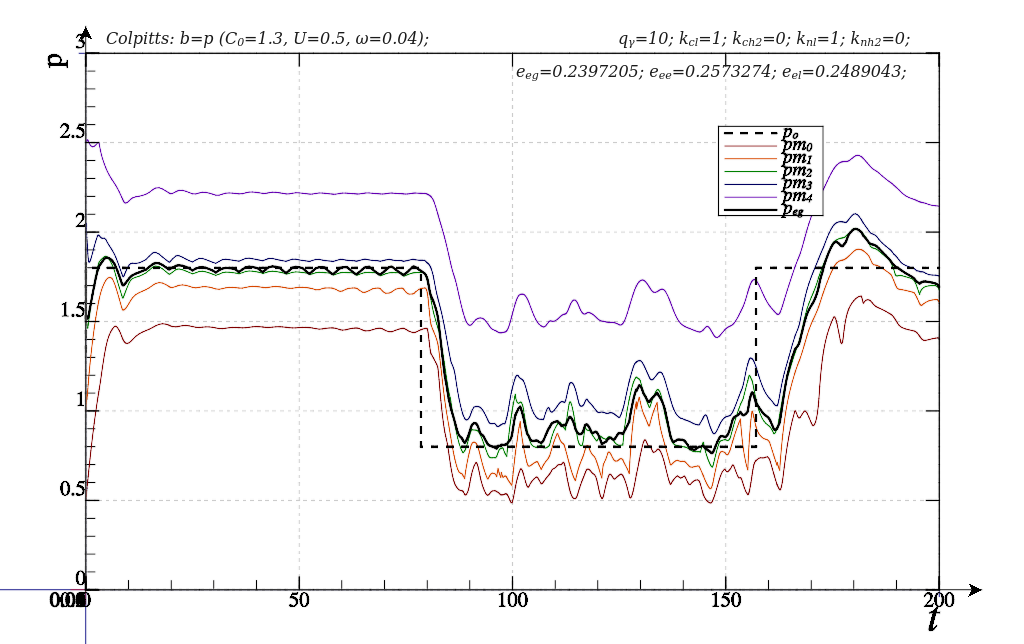
\includegraphics[width=0.49\textwidth]{p/cha/colp/colp_m5p-pl_n_sign.png}
  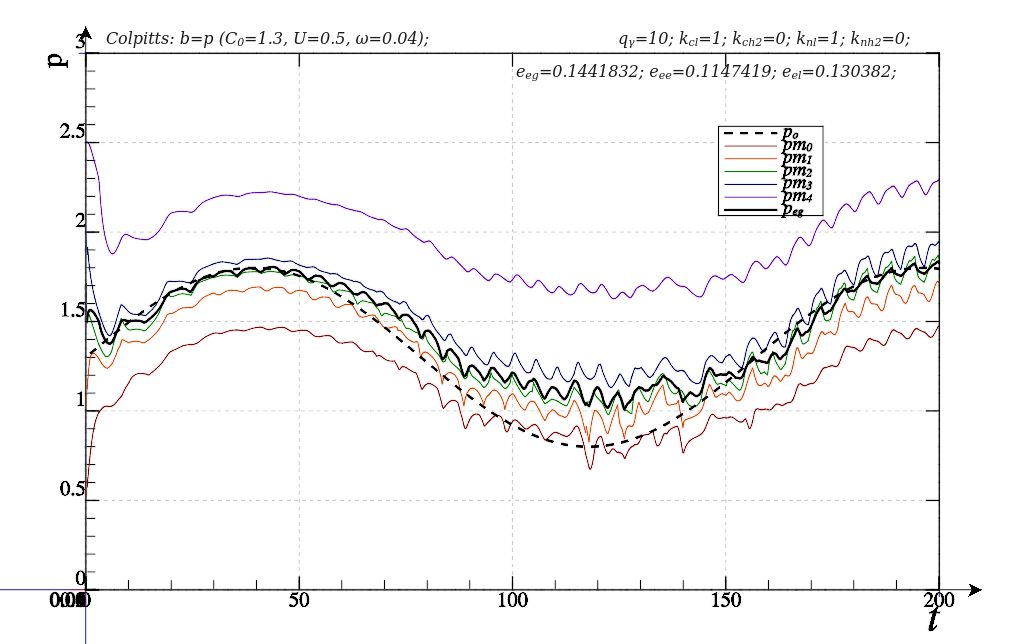
\includegraphics[width=0.49\textwidth]{p/cha/colp/colp_m5p-pl_n_sin.png}
}
\caption{Процесс идентификации параметра $b$ системы (\ref{atu:eq:colp})
  при условиях (\ref{atu:eq:colp_b_sign}) и (\ref{atu:eq:colp_b_sin})
}
\label{atu:f:colp_id}
\end{figure}

Зависимость среднеквадратических ошибок идентификации от величины $q_\gamma$ (рис.~\ref{atu:f:colp_e_qgamma})
даёт информацию о правильной настройке этого параметра системы идентификации.

\begin{figure}[htb!]
\centerline{
  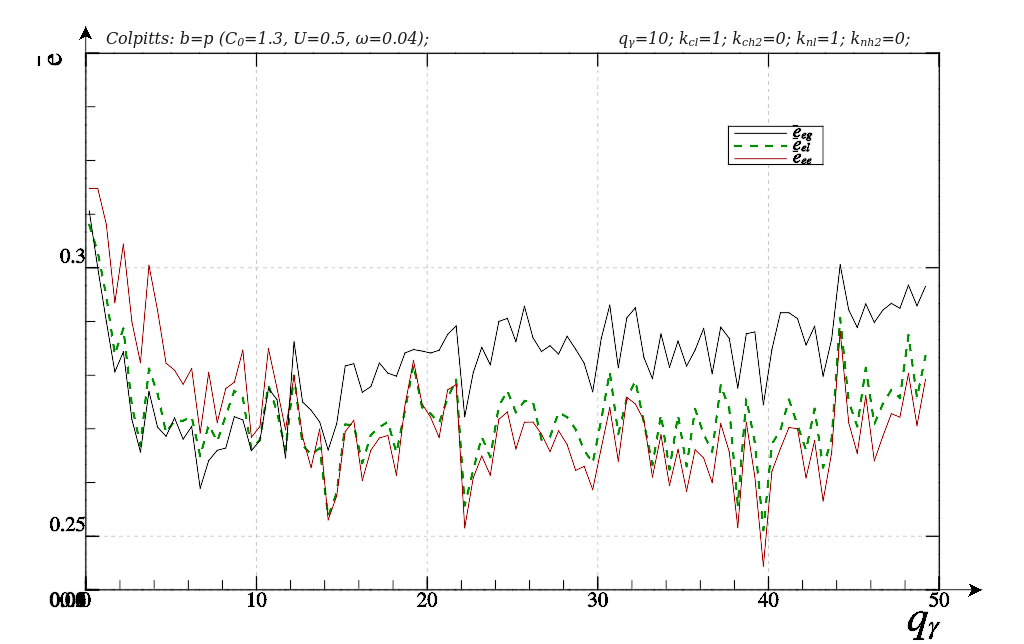
\includegraphics[width=0.49\textwidth]{p/cha/colp/colp_m5p-p_qg_e_sign.png}
  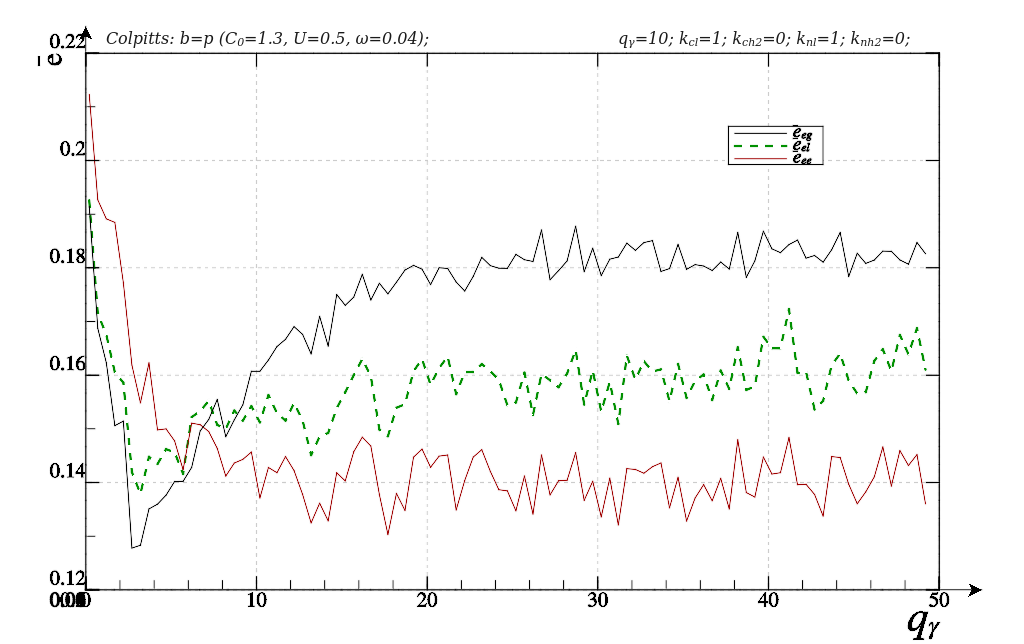
\includegraphics[width=0.49\textwidth]{p/cha/colp/colp_m5p-p_qg_e_sin.png}
}
  \caption{Зависимости  $\bar{e}(q_\gamma)$ для системы (\ref{atu:eq:colp})
  при условиях (\ref{atu:eq:colp_b_sign}) и (\ref{atu:eq:colp_b_sin})
}
\label{atu:f:colp_e_qgamma}
\end{figure}



Аналогично, зависимости $\bar{e_*}(a_q)$ (рис.~\ref{atu:f:colp_e_a_q})
позволяют корректно определить время усреденения.
Полученные результаты хорошо согласуются со спектрами системы.

\begin{figure}[htb!]
\centerline{
  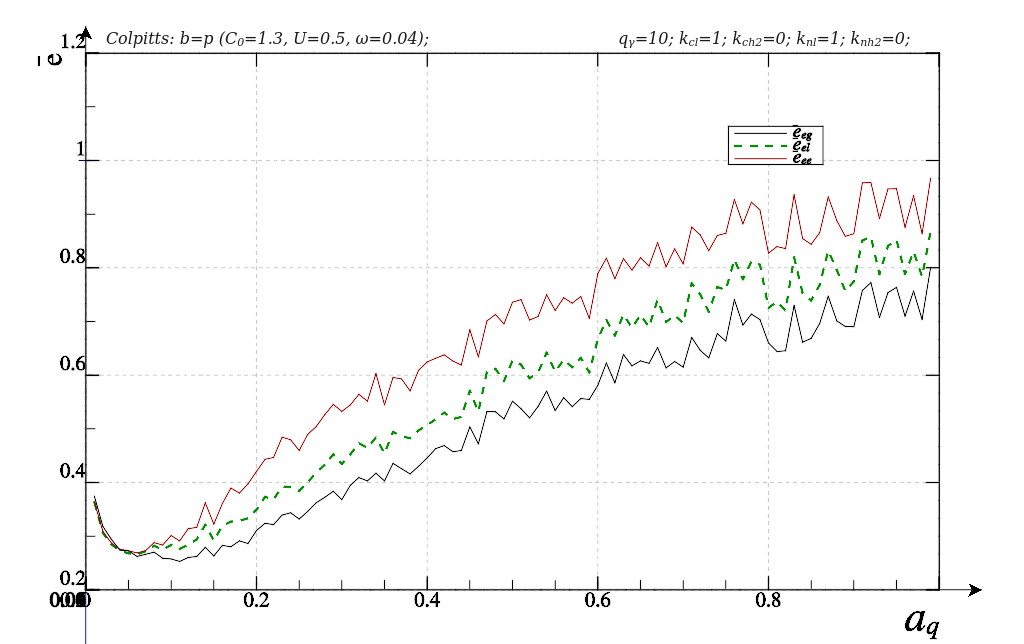
\includegraphics[width=0.49\textwidth]{p/cha/colp/colp_m5p-p_a_q_e_sign.png}
  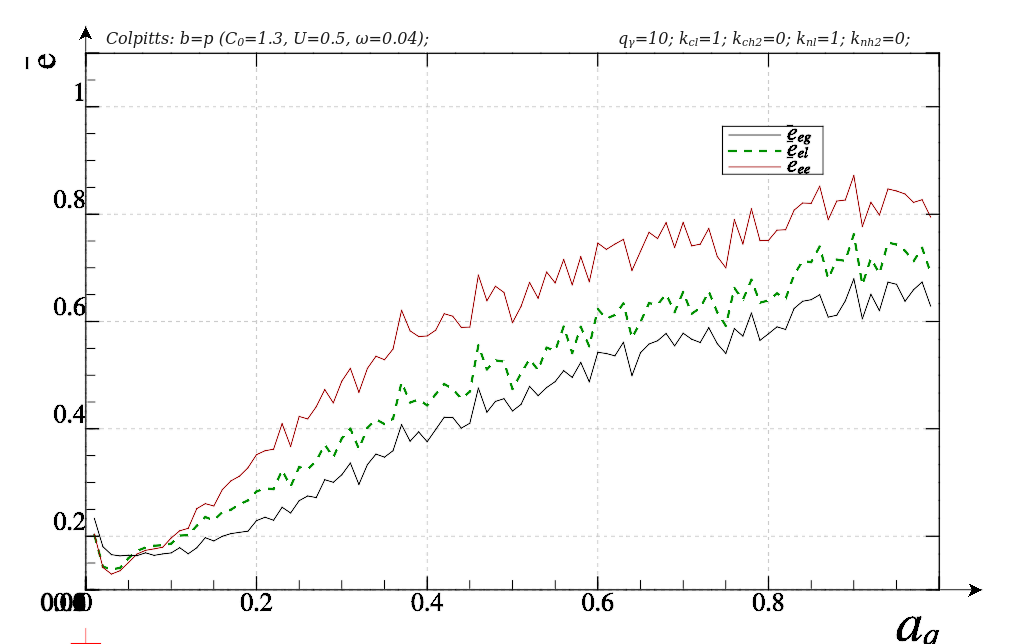
\includegraphics[width=0.49\textwidth]{p/cha/colp/colp_m5p-p_a_q_e_sin.png}
}
  \caption{Зависимости  $\bar{e}(a_q)$ для системы (\ref{atu:eq:colp})
  при условиях (\ref{atu:eq:colp_b_sign}) и (\ref{atu:eq:colp_b_sin})
}
\label{atu:f:colp_e_a_q}
\end{figure}

В целом синтез критерия идентификации, и построение работоспособной системы идентификации для
системы Колпитца не потребовало никаких специальных подходов.


\FloatBarrier

\subsubsection{Колебательная с зоной нечувствительности в возвращающей силе} % _DEADVI_

\LinkRef{
  deadvi: ASAU-20, ISDMCI-2013
}

\begin{equation}
\ddot{x} + c_0 \dot{x} + a \cdot x + b \cdot \mathrm{db}(x,x_0) = u(t),
\label{atu:eq:deadvi}
\end{equation}

$ u(t) = U_0 \sin( \omega_{in} t ) $.

Идентифицируемый параметр:
$ x_0 \in [2;2.5] $ -- ширина зоны нечувствительности.

Остальные параметры:
$U_0 = 1.4$, $\omega_{in} = 1.4$, $c_0=0.1$, $a=-0.3$, $b=1.0$.


\begin{figure}[htb!]
\centerline{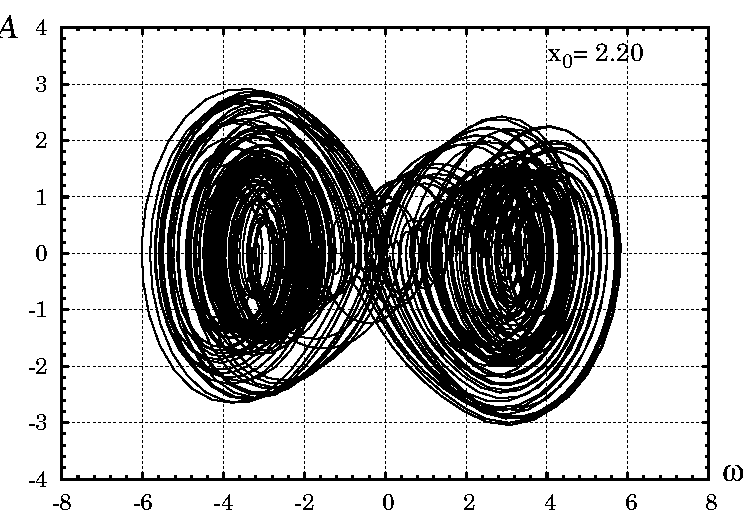
\includegraphics[width=0.5\textwidth]{p/cha/deadvi_phase.pdf} }
\caption{Фазовый портрет системы ``deadvi'' (\ref{atu:eq:deadvi})}
\label{atu:f:deadvi_phase}
\end{figure}

Критерий
$\overline{x^2(t)}$


\FloatBarrier
\subsubsection{Система Sprott A}

\LinkRef{
  spr\_a: MKMM-2016
}

В своих работах J.C.~Sprott рассмотрел целое семейство динамических
систем, реализующих хаотическое поведение, обозначив их латинскими буквами
от ``A'' до ``S''~[??]. Особое место среди них
занимает система, обозначаемая как ``Sprott A''. Отличительной особенностью
этой системы является отсутствие положений равновесия, что делает
невозможным применение многих известных методов анализа, основанных на
каком-либо разложении в окрестностях точек равновесия. Соответствующая ей
система уравнений имеет вид:

\begin{equation}
  \begin{cases}
    \dot{x} =  y, \\
    \dot{y} = -x + yz, \\
    \dot{z} =  1 - y^2.
  \end{cases}
  \label{atu:eq:spr_a_orig}
\end{equation}


В исходном виде система (\ref{atu:eq:spr_a_orig}) имеет фиксированные значения параметров.
Не изменяя структуры системы, можно ввести 5 параметров, влияющие на её динамку. В
данной работе рассмотрим только один -- $c_{x_y} $. Система принимает следующий вид:

\begin{equation}
  \begin{cases}
    \dot{x} =  c_{x_y} y, \\
    \dot{y} = -x + yz, \\
    \dot{z} =  1 - y^2.
  \end{cases}
  \label{atu:eq:spr_a}
\end{equation}

В таком виде система, при изменении $c_{x_y} $
в достаточно широком диапазоне может демонстрировать как
сложно-периодическое, так и преимущественно, хаотическое
поведение (рис.~\ref{atu:f:spr_a_phase}). При этом, в диапазоне $c_{x_y} \in [0.1 ; 0.7] $
наблюдаются перестройки структуры аттрактора, а при относительно больших
значениях данного параметра аттрактор представляет собой полый тор.


\begin{figure}[htb!]
\centerline{
  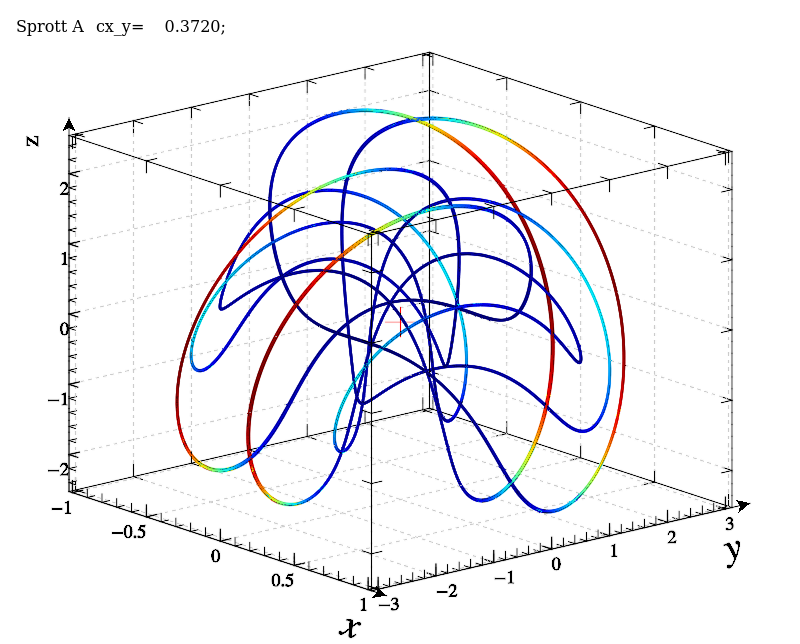
\includegraphics[width=0.33\textwidth]{p/cha/spr_a/sprott_a-p_xyz_cx_y=0x372.png}
  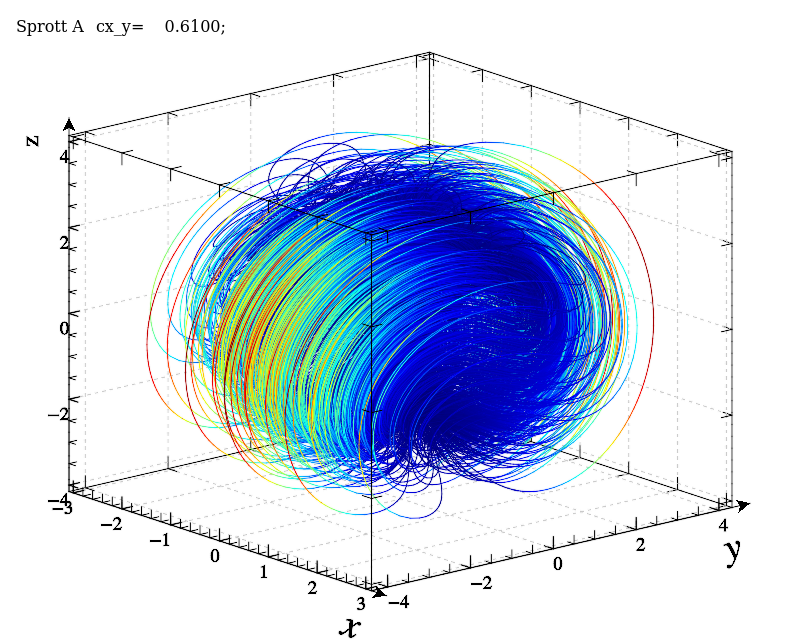
\includegraphics[width=0.33\textwidth]{p/cha/spr_a/sprott_a-p_xyz_cx_y=0x610.png}
  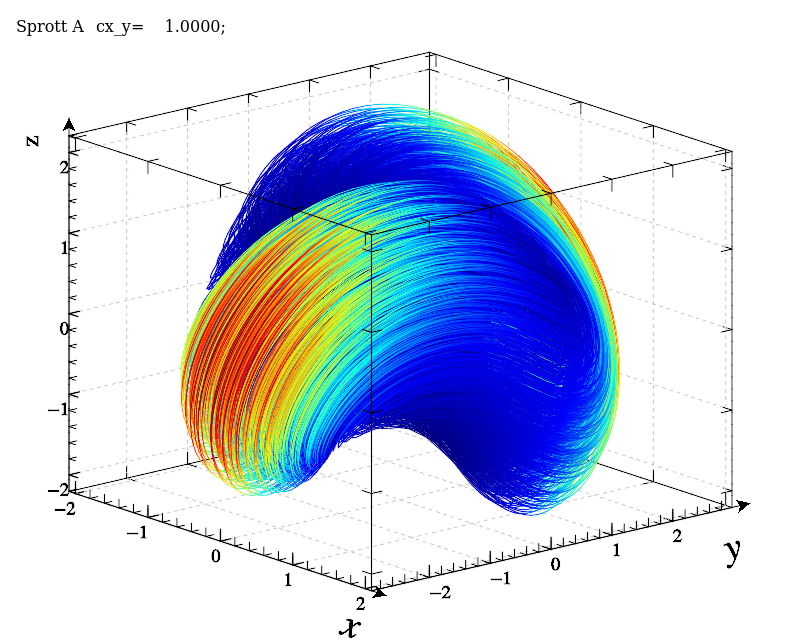
\includegraphics[width=0.33\textwidth]{p/cha/spr_a/sprott_a-p_xyz_cx_y=1x000.png}
}
\caption{Аттракторы системы (\ref{atu:eq:spr_a})
  при $ c_{x_y} =0.372 $, $ c_{x_y} =0.61 $, $ c_{x_y} =1.00 $
}
\label{atu:f:spr_a_phase}
\end{figure}

Важной особенностью поведения этой системы что при $ c_{x_y} \ge 1 $
в спектре системы имеются очень ограниченные участки сплошного спектра~(рис.~\ref{atu:f:spr_a_f}).
При этом, как и для получения корректного спектра, так и для обнаружения разбегания траекторий
необходимо моделирование системы на протяжении достаточно длительного
(по сравнению с многими схожими системами) модельного времени.

\begin{figure}[htb!]
\centerline{
  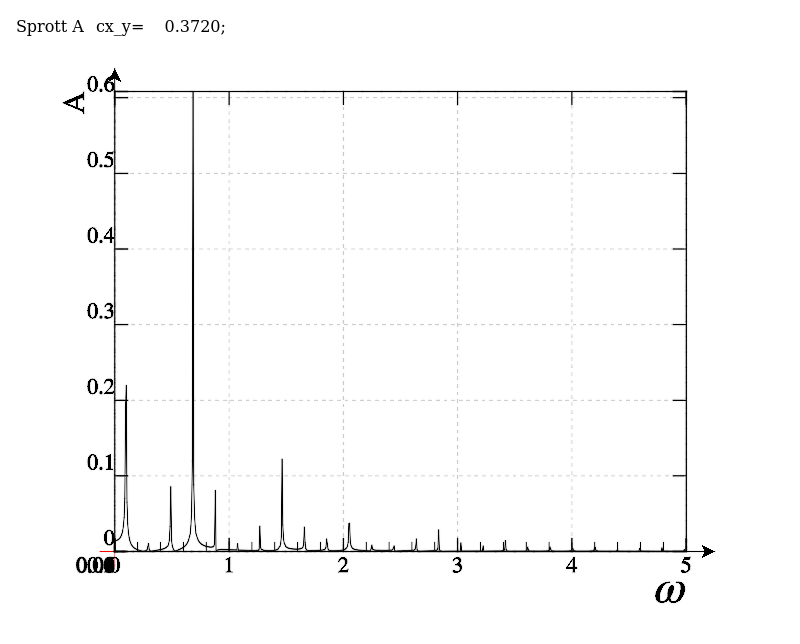
\includegraphics[width=0.33\textwidth]{p/cha/spr_a/sprott_a_f-p_f_cx_y=0x372.png}
  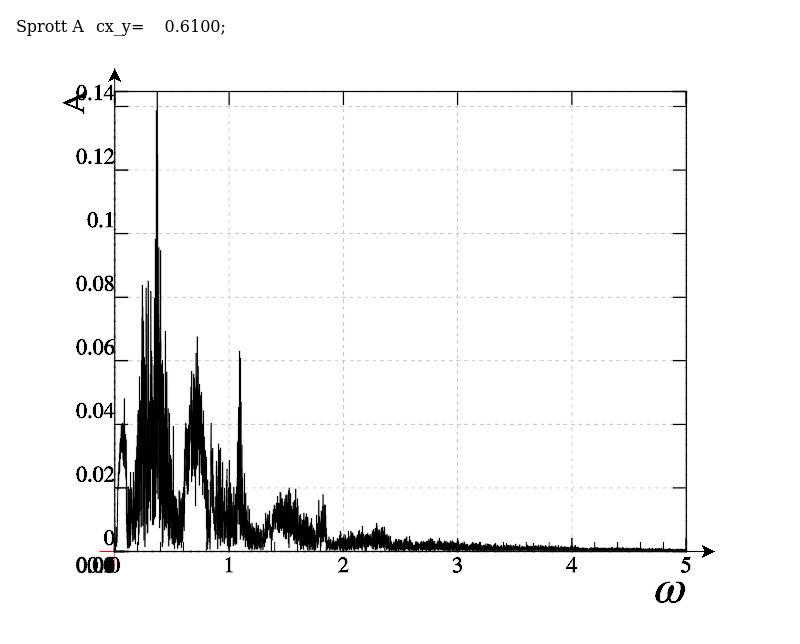
\includegraphics[width=0.33\textwidth]{p/cha/spr_a/sprott_a_f-p_f_cx_y=0x610.png}
  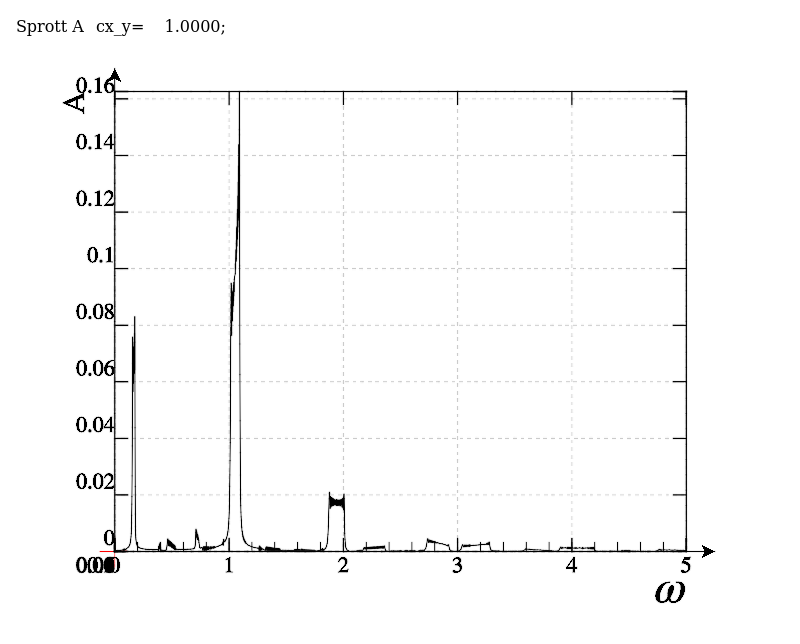
\includegraphics[width=0.33\textwidth]{p/cha/spr_a/sprott_a_f-p_f_cx_y=1x000.png}
}
\caption{Спектры системы (\ref{atu:eq:spr_a})
  при $ c_{x_y} =0.372 $, $ c_{x_y} =0.61 $, $ c_{x_y} =1.00 $
}
\label{atu:f:spr_a_f}
\end{figure}

Рассмотрим зависимости $q_{*}(c_{x_y}) $ (рис.~\ref{atu:f:spr_a_q})
для системы (\ref{atu:eq:spr_a}). Анализ зависимостей
даёт однозначный ответ о возможном виде критерия -- $q_{x^2}$.
Используя его, строим систему идентификации.

\begin{figure}[htb!]
\centerline{
  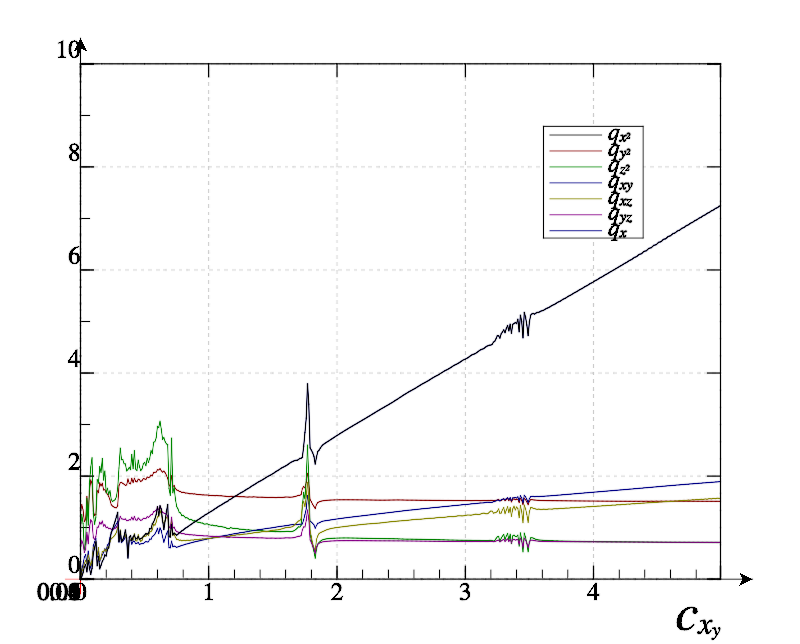
\includegraphics[width=0.50\textwidth]{p/cha/spr_a/sprott_a_p-p_c_x_y.png}
}
\caption{Зависимости $q_{*}(c_{x_y})$ для системы (\ref{atu:eq:spr_a}) }
\label{atu:f:spr_a_q}
\end{figure}


Динамика процессов идентификации для системы Sprott A представлена на рис.~\ref{atu:f:spr_a_id}.
Общий вид динамики поиска свидетельствует о работоспособности системы.

\begin{figure}[htb!]
\centerline{
  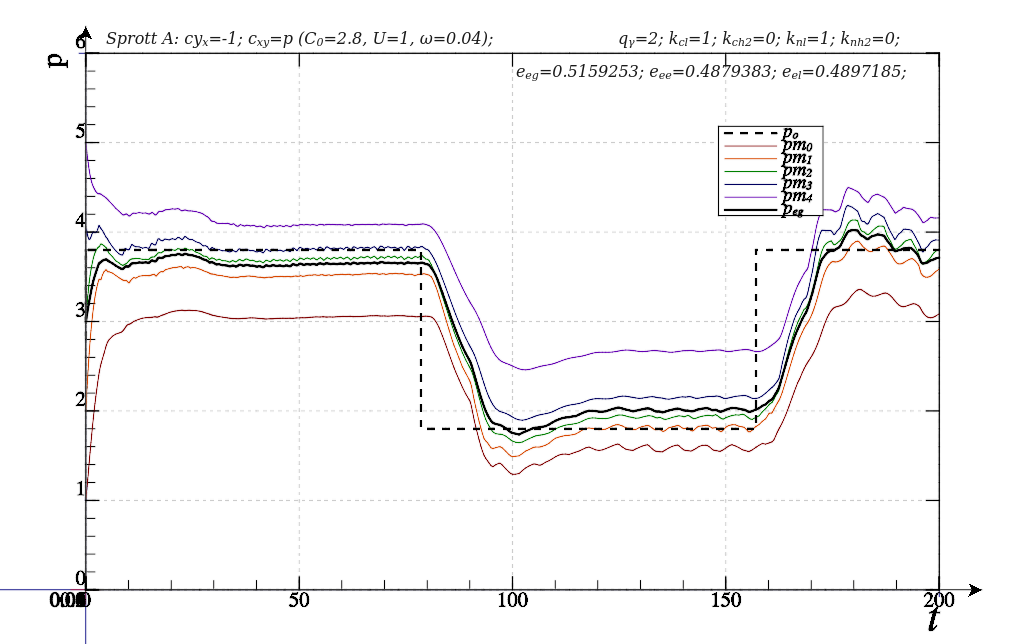
\includegraphics[width=0.49\textwidth]{p/cha/spr_a/sprott_a_m5p-pl_n_sign.png}
  \includegraphics[width=0.49\textwidth]{p/cha/spr_a/sprott_a_m5p-pl_n_sin.png}
}
\caption{Процесс идентификации параметра $c_{x_y} $ системы (\ref{atu:eq:spr_a})
  при различных видах нестационарности этого параметра
}
\label{atu:f:spr_a_id}
\end{figure}

Зависимость среднеквадратических ошибок идентификации от величины $q_\gamma$ (рис.~\ref{atu:f:spr_a_e_qgamma})
свидетельствует о довольно слабой зависимости (в разумных пределах)
динамики системы идентификации о  этого параметра. Скорее всего,
здесь проявляются робастные свойства поисковых агентов.

\begin{figure}[htb!]
\centerline{
  \includegraphics[width=0.49\textwidth]{p/cha/spr_a/sprott_a_m5p-p_qg_e_sign.png}
  \includegraphics[width=0.49\textwidth]{p/cha/spr_a/sprott_a_m5p-p_qg_e_sin.png}
}
  \caption{Зависимости  $\bar{e}(q_\gamma)$ для системы (\ref{atu:eq:spr_a})
  при различных видах нестационарности этого параметра
}
\label{atu:f:spr_a_e_qgamma}
\end{figure}


Зависимости $\bar{e_*}(a_q)$ (рис.~\ref{atu:f:spr_a_e_a_q})
с одной стороны, позволяют корректно определить время усреденения,
с другой -- подтверждают тезис о том, что более ярко выраженной изменение
параметра требует большего времени наблюдения за системой
для проведения идентификации.

\begin{figure}[htb!]
\centerline{
  \includegraphics[width=0.49\textwidth]{p/cha/spr_a/sprott_a_m5p-p_a_q_e_sign.png}
  \includegraphics[width=0.49\textwidth]{p/cha/spr_a/sprott_a_m5p-p_a_q_e_sin.png}
}
  \caption{Зависимости  $\bar{e}(a_q)$ для системы (\ref{atu:eq:spr_a})
  при различных видах нестационарности этого параметра
}
\label{atu:f:spr_a_e_a_q}
\end{figure}

И в этом случае удалось создать и критерий идентификации, и работоспособную систему идентификации
на основании энергетического критерия.



\FloatBarrier
\subsubsection{Система с сухим трением} % __FRIC__

\LinkRef{
  fric: ASAU-11, DSMP-2016
}

Существуют динамические системы, не обладающие хаотическим поведением,
которые, тем не менее, проявляют сходные свойства с точки зрения идентификации.
А именно, непосредственное сравнение выходов системы и модели не позволяет
сделать никаких выводов о соотношениях между параметрами модели о объекта.
Одним из примеров является динамическая система, моделирующая поведение
тела заданной массы по действием внешней вынуждающей силы и силы сухого трения (\ref{atu:eq:dryfric_sys}):

\begin{equation}
 m \ddot{x} + f( x, \dot{x}, \ldots)  = u(t).
\label{atu:eq:dryfric_sys}
\end{equation}

\noindent
где
$m$ -- масса тела,
$u(t)$ -- вынуждающая сила,
$ f( x, \dot{x}, \ldots)  $ -- сила сухого трения.

Важной особенностью при моделировании силы сухого трения является тот факт,
это это силу невозможно корректно выразить аналитически. Более того,
её алгоритмическое представления неизбежно потребует учёта всех других сил,
действующих на тело, то крайней мере, для корректного представления
силы трения покоя. Эта особенность не даёт возможности
аналитического анализа таких систем, за исключением ограниченного набора
вырожденных случаев. При этом, такое поведение существенно затрудняет идентификацию,
и в определённых случаях делает её принципиально невозможной.

Основным параметром, в простейшем случае определяющим силу сухого
трения, является $f_{dm}$ -- максимальная значение её модуля.
Определение этой величины и будем считать целью задачи идентификации.

Существенным свойством данной системы является то, что в каждой точке \(x\)
система может находится в покое, даже если на неё действует
внешняя сила (по модулю не превышающая $f_{dm}$).
Если же рассмотреть пару или более подобных систем,
то получившаяся система имеет общие свойства с системами
хаотической динамики, а именно: малые возмущения входного сигнала
или коэффициентов модели приводят к значительным изменениям
выходного, причем реакция на возмущения может быть
не ограничена во времени.
Более того, если после какого-то момента времени
параметры объекта и коэффициенты модели полностью совпадут,
величина ошибки выходных не устремится к нулю, а останется на прежнем уровне.

На рис.~\ref{atu:f:fric_outs} представлен сравнительный пример динамики трёх
моделей, при одинаковом входном сигнале
и различных значениях $f_{dm}$.

\begin{figure}[htb!]
  \centerline{
    \includegraphics[width=0.5\textwidth]{p/cha/fric/fric_outs.png}
  }
  \caption{Динамика трёх моделей вида (\ref{atu:eq:dryfric_sys})}
  \label{atu:f:fric_outs}
\end{figure}

При дальнейшем моделировании, в качестве сигнала $u(t)$ использовался кусочно-линейный периодический сигнал,
в котором чередуются ``плато'' и резкие изменения. Выбор такая форма обусловлен
характерными режимами работы систем позиционирования электромеханических
устройств, для которых и характерно влияние сухого трения.

Для обеспечения возможности применения методов идентификации,
необходимо существование критерия идентификации
\( q(x(t)) \),
удовлетворяющего следующим требованиям:

\begin{itemize}

\item
чувствительность к \textit{динамике} модели и объекта;

\item
свойство астатизма, то есть
независимость
от смещения выхода объекта или модели:
\( q(x(t)+a ) \approx q( x(t) ) \);

\item
достаточная устойчивостью к шумам измерения;

\item
физическая реализуемость.

\end{itemize}

Первые два требования
могут быть достигнуты путём вычисления производной --
скорости изменения выходных сигналов
\(v = dx(t)/dt \),
и формирования критерия идентификации на её основе.

Однако, при этом система становится исключительно чувствительной
к шумам измерения. Даже в том случае, когда
оценка производной производится физически реализуемыми методами,
создать работоспособную систему идентификации на основе критериев
подобного вида практически невозможно.

В работе [asau11??] был предложен метод синтеза критерия идентификации
на основе гистерезисной фильтрации выходных сигналов, с последующим
вычислением производной. Метод показал свою работоспособность, однако,
он требует достаточно точных сведений об уровне и шумов шумов -- для
настройки гистерезисного фильтра. В данной работе сделаем предположение,
что уровень шумов позволяет создать фильтр, позволяющий отсеивать шумы
за (как максимум) характерное время реакции системы.
После фильтра действует реальное дифференцирующее звено.
Соответствующий вид критерия обозначим как $ q_{dx} $ (рис.~\ref{atu:f:fric_q}).



\begin{figure}[htb!]
\centerline{
  \includegraphics[width=0.50\textwidth]{p/cha/fric/fric_p-p_f_dm_q.png}
}
  \caption{Зависимость $q_{dx}(f_{dm})$ для системы (\ref{atu:eq:dryfric_sys}) }
\label{atu:f:fric_q}
\end{figure}


Динамика процессов идентификации для системы (\ref{atu:eq:dryfric_sys}) представлена на рис.~\ref{atu:f:spr_a_id}.
Следует отметить сильное влияние входного сигнала, так как когда системы неподвижны
на одном из ``плато'', то нет возможности различить из параметры,
какой бы критерий не использовался.

\begin{figure}[htb!]
\centerline{
  \includegraphics[width=0.49\textwidth]{p/cha/fric/fric_m5p-pl_n_sign.png}
  \includegraphics[width=0.49\textwidth]{p/cha/fric/fric_m5p-pl_n_sin.png}
}
\caption{Процесс идентификации параметра $c_{x_y} $ системы (\ref{atu:eq:dryfric_sys})
  при различных видах нестационарности этого параметра
}
\label{atu:f:fric_id}
\end{figure}

Зависимость среднеквадратических ошибок идентификации от величины $q_\gamma$ (рис.~\ref{atu:f:fric_e_qgamma})
достаточно сильно отличатся от аналогичной, например, для системы ``Sprott A''. На ней явно выражены
экстремумы, дающие возможность тонкой настройки системы идентификации. Следовательно,
для данной динамической системы робастные свойства системы идентификации проявляются слабо,
и может потребовался дополнительная адаптация.

\begin{figure}[htb!]
\centerline{
  \includegraphics[width=0.49\textwidth]{p/cha/fric/fric_m5p-p_qg_e_sign.png}
  \includegraphics[width=0.49\textwidth]{p/cha/fric/fric_m5p-p_qg_e_sin.png}
}
  \caption{Зависимости  $\bar{e}(q_\gamma)$ для системы (\ref{atu:eq:dryfric_sys})
  при различных видах нестационарности этого параметра
}
\label{atu:f:fric_e_qgamma}
\end{figure}


Зависимости $\bar{e_*}(a_q)$ (рис.~\ref{atu:f:fric_e_a_q})
 позволяют корректно определить время усреденения.

\begin{figure}[htb!]
\centerline{
  \includegraphics[width=0.49\textwidth]{p/cha/fric/fric_m5p-p_a_q_e_sign.png}
  \includegraphics[width=0.49\textwidth]{p/cha/fric/fric_m5p-p_a_q_e_sin.png}
}
  \caption{Зависимости  $\bar{e}(a_q)$ для системы (\ref{atu:eq:dryfric_sys})
  при различных видах нестационарности этого параметра
}
\label{atu:f:fric_e_a_q}
\end{figure}

Для данной системы энергетические критерии, аналогичные применённым в предыдущих случаях,
оказались неприменимы. Критерий, хоть и основанный на измерении производной (после фильтрации),
оказался работоспособным. В первую очередь это связано с тем, что в основе были положены
физические принципы, которые для данной системы вполне очевидны.





\FloatBarrier
\subsubsection{Релаксационные генераторы}


\LinkRef{
  relax: ASAU-18 (no id?)
}

\begin{figure}[htb!]
\centerline{\includegraphics[width=0.5\textwidth]{p/cha/relax_phase3_0500.pdf} }
\caption{Аттрактор системы с релаксационными генераторами}
\label{atu:f:relax_phase3}
\end{figure}



\FloatBarrier
\subsubsection{VGlass} % _VGLASS_

\LinkRef{
  vglass: ITMM-2013
}

\begin{figure}[htb!]
\centerline{\includegraphics[width=0.5\textwidth]{p/cha/vg1-graph_phase.png} }
\caption{Фазовый портрет системы ``vglass'' }
\label{atu:f:vglass_phase}
\end{figure}


\FloatBarrier
\subsubsection{Common}

Фрактальные критерии (инвариантные относительно смены частоты дискретизации)?
Надо ли несколько критериев, если параметров несколько.
А может надо, даже если один?

Структуры ...



\FloatBarrier
\section{Методы поиска}

\subsection{Основные параметры поиска}


\subsubsection{Общие свойства объектов с точки зрения идентификации}

\subsubsection{Априорная и текущая информация}

Без априорной информации невозможно построение
работоспособной системы идентификации. Основные
априорные величины определяются на этапе постановки
задачи идентификации. В первую очередь это
параметры масштаба: допустимый диапазон
изменения параметров \( \mathfrak{P}\),
характерное время работы
идентифицируемой системы, а также
требуемая точность и скорость идентификации
(могут быть заданы различными способами).
В этот список входи и максимальная скорость изменения параметра.
В процессе работы эти параметры могут уточнятся по текущей информации.

Следующую часть априорной (по отношению к идентификации) информации
предоставляет процесс синтеза критерия идентификации.
В первую очередь, это сам вид критерия. Им определятся
как диапазон изменения величины этого критерия, так и
динамические свойства: характерное/минимально время
оценивали \(\tau\) (или даже оценка зависимости $\tau$ от точности и других параметров),
характерное время реакции системы на изменение
параметра с учётом динамики измерения \(q\).


\subsubsection{Чувствительность модели}

Убрать или заменить чем-то ещё.


\subsection{Время и история}

Способы учёта истории системы и динамических характеристик.

\subsection{ Использование множества моделей / агентов}

Сколько всего надо моделей? Размер пространства параметров.
Рой, коллектив, главнюк.
Зачем агентам перемещаться?

\textbf{ Агент } -- совокупность модели, критерия идентификации,
алгоритмов поиска и адаптации.

Как правило, один агент управляет одной моделью. При этом
он может использовать информацию, как полученную как от других
агентов, так и полученную в результате обработки данных
всего ансамбля.

\textbf{ Рой } -- множество агентов, обеспечивающее идентификацию за счёт
сосредоточения максимального количества агентов
в области предполагаемого максимума функции качества.
Обычно -- три составляющие поведения
(движение о оцениваемому локальному экстремуму, -- к глобальному, случайная составляющая).

\Cmt{Для сравнения требуется и это промоделировать.
Достаточно накладно -- надо много агентов.}

Достоинства -- простота алгоритмов.
Недостатки -- требуется избыточное количество агентов.
Значительная часть агентов, находящихся вблизи экстремума,
практически не приносит информации. Роевые
алгоритмы (как и их прообразы в живой природе) ориентированы
для увеличения добычи ресурсов, а не информации.

\textbf{ Ансамбль } -- множество агентов, обеспечивающее идентификацию за счёт
распределения агентов таким образом, который обеспечивает как
точность идентификации за счёт ограниченного скопления агентов
в областях предполагаемых максимумов, так и оперативное переключение
на другие области при изменении параметров за счёт недопущения
неоправданной скученности агентов.

\Cmt{ Заметная часть новизны планируется здесь}

\subsubsection{Один агент}

Единственный неподвижный агент практически не имеет смысла
с точки зрения синтеза системы идентификации.
Он может сигнализировать о том, что в пределах
\(\tau\) модель была или не была достаточно адекватна
объекту.

Наличие истории и возможность перемещаться дают возможность
построить систему идентификации и на одном агенте.
В качестве истории могут использоваться, в том числе,
динамические свойства идентифицируемого объекта
(оригинальный метод АПИ). Также могут быть
применены интегрирующие элементы агента идентификации
(синхронный детектор, \ldots).

\subsubsection{Пара агентов}

Пара агентов, взаимодействующая между собой,
способна оценить градиент функции качества,
и, следовательно, обеспечить смещение в требуемом направлении.

С учетом глобальной информации возможна адаптация параметров пары.
В свою очередь, информация, полученная от пары может
использоваться для уточнения глобальных параметров.

\subsubsection{Триплет агентов}

Три соседних агента, взаимодействующие между собой,
способны не только оценить градиент функции качества в своей окрестности,
но и определить (опять же, оценочно) наличие там максимума.

\subsubsection{Ансамбль агентов}

\subsection{Адаптация}

\Cmt{
Какие параметры системы идентификации можно адаптировать
и на каком уровне.

Когда имеет смысл играть с чувствительностью.

Как близко имеет смысл подводить модели к экстремуму?
}


Стабильные/мобильные модели.

История: локальная + глобальная

\subsection{Качество идентификации}

\Cmt{Расширить из кандидатской с учётом времени и множества моделей.}



\section{Программная реализация}

\subsection{Постановка задачи}

\Cmt{Из того, что получится \ldots}

\subsection{Структура программного комплекса}

Комплекс -- потому что несколько программ.
От основной для моделирования, до программ сбора и обработки
информации для микроконтроллеров.

\subsection{Взаимодействие с реальным миром}

\Cmt{
Просто прочитать данные - уже работает.
Надо: realtime.
Протокол(ы) взаимодействия (+ существующие).
}


\section{Реальные задачи}

\Cmt{
Ага....
}


%\section{Всякое и старое}



%Как надо крутить $\tau_g$ вблизи/вдали
% 1) При малом $k_\omega$ сравнить поведение вблизи/вдали при различном $\omega_0$
% 2) Двойная инверсия работы генератора?

%Две точки усреднения: как объединить? А надо ли?

%Адаптация $\tau_q$ / просто $\tau$ от $x$.





\end{document}

